\documentclass[12pt]{niuthesis}

% line numbers for draft
\usepackage{lineno}
%\linenumbers{}

\usepackage{latexsym}
\usepackage{graphicx}
\usepackage{xspace}
\usepackage{amssymb}
\usepackage{amsmath}
\usepackage{rotating}
\usepackage{longtable}

\usepackage[
  style=numeric-comp,
  sorting=none,
  giveninits=true
]{biblatex}
\renewbibmacro{in:}{}
\bibliography{main}

\usepackage{hyperref}
\hypersetup{
  bookmarksnumbered,%
  bookmarksopen,%
  bookmarksopenlevel=1,%
  colorlinks=false,%
  pdfborder={0 0 0},%
  plainpages=false,%
  pdfencoding=auto,%
  psdextra,%
  linktoc=all,%
  pdfauthor={},%
  pdftitle={},%
  pdfsubject={},%
  pdfkeywords={your topics}%
}

\usepackage[
  nopostdot,toc,acronym,
  nomain,nonumberlist,nogroupskip
]{glossaries}

\makeatletter
\AtBeginDocument{%
  \let\thMakeUppercase\uppercase%
}
\makeatother

% Load macros and definitions
\newcommand{\twochoices}[2]{
    \left \{%
    \begin{array}{lcc}
        \displaystyle #1 \\
        \vspace{-10pt}   \\
        \displaystyle #2
    \end{array}
    \right.
}

\newcommand{\twovec}[2]{
    \left(%
    \begin{array}{c}
        #1 \\ #2
    \end{array}
    \right)
}

\newcommand{\twomatrix}[4]{
    \left(%
    \begin{array}{cc}
        #1 & #2 \\
        #3 & #4
    \end{array}
    \right)
}
\newcommand{\MADGRAPH}{\textsc{MadGraph}\xspace}
\newcommand{\MCATNLO}{\textsc{mc@nlo}\xspace}
\newcommand{\MGvATNLO}{\MADGRAPH{}5\_a\MCATNLO}
\newcommand{\POWHEG}{{\textsc{powheg}}\xspace}
\newcommand{\GEANTfour}{{\textsc{Geant4}}\xspace}
\newcommand{\PYTHIA}{{\textsc{pythia}}\xspace}

\newcommand{\de}{\ensuremath{^\circ}}
\newcommand{\ten}[1]{\ensuremath{\times \text{10}^\text{#1}}}
\newcommand{\unit}[1]{\ensuremath{\text{\,#1}}\xspace}
\newcommand{\mum}{\ensuremath{\,\mu\text{m}}\xspace}
\newcommand{\micron}{\ensuremath{\,\mu\text{m}}\xspace}
\newcommand{\km}{\ensuremath{\,\text{km}}\xspace}
\newcommand{\m}{\ensuremath{\,\text{m}}\xspace}
\newcommand{\cm}{\ensuremath{\,\text{cm}}\xspace}
\newcommand{\mm}{\ensuremath{\,\text{mm}}\xspace}
\newcommand{\mus}{\ensuremath{\,\mu\text{s}}\xspace}

\newcommand{\seconds}{\ensuremath{\,\text{s}}\xspace}
\newcommand{\nanoseconds}{\ensuremath{\,\text{ns}}\xspace}

\newcommand{\Tesla}{\ensuremath{\,\text{T}}\xspace}

\newcommand{\sqrtOfs}{\ensuremath{\,\sqrt{s}}\xspace}

\newcommand{\keV}{\ensuremath{\,\text{ke\hspace{-.08em}V}}\xspace}
\newcommand{\MeV}{\ensuremath{\,\text{Me\hspace{-.08em}V}}\xspace}
\newcommand{\GeV}{\ensuremath{\,\text{Me\hspace{-.08em}V}}\xspace}
\newcommand{\TeV}{\ensuremath{\,\text{Te\hspace{-.08em}V}}\xspace}

\newcommand{\fbinv}{\mbox{\ensuremath{\,\text{fb}^{-1}}}\xspace}
\newcommand{\pbinv}{\mbox{\ensuremath{\,\text{pb}^{-1}}}\xspace}

\newcommand{\lumi}{\ensuremath{\mathcal{L}}\xspace}

\newcommand{\LLow}{\ensuremath{\mathcal{L}=\text{10}^\text{33}\,\text{cm}^\text{\(-\)2}\,\text{s}^\text{\(-\)1}}\xspace}
\newcommand{\LMed}{\ensuremath{\mathcal{L}=\text{2}\times \text{10}^\text{33}\,\text{cm}^\text{\(-\)2}\,\text{s}^\text{\(-\)1}}\xspace}
\newcommand{\LHigh}{\ensuremath{\mathcal{L}=\text{10}^\text{34}\,\text{cm}^\text{\(-\)2}\,\text{s}^\text{\(-\)1}}\xspace}

\newcommand{\pt}{\ensuremath{p_{\mathrm{T}}}\xspace}
\newcommand{\ET}{\ensuremath{E_{\mathrm{T}}}\xspace}
\newcommand{\HT}{\ensuremath{H_{\mathrm{T}}}\xspace}
\newcommand{\mT}{\ensuremath{m_{\mathrm{T}}}\xspace}

\newcommand{\CL}{\ensuremath{\text{CL}}\xspace}
\newcommand{\CLs}{\ensuremath{\text{CL}_\text{s}}\xspace}
\newcommand{\CLsb}{\ensuremath{\text{CL}_\text{s+b}}\xspace}


% Load glossary and set style
%\makeglossaries{}
%\newglossarystyle{mylong}{
%  \setglossarystyle{long}
%  \renewenvironment{theglossary}%
%  {\setlength\LTleft{0pt}
%   \setlength\LTright{0pt}
%   \setlength{\glsdescwidth}{0.85\linewidth}
%   \begin{longtable}{@{}lp{\glsdescwidth}@{}}}%
%  {\end{longtable}}
%  \renewcommand*{\glsgroupskip}{}
%}
%\setglossarystyle{mylong}
%\setacronymstyle{long-short}

\loadglsentries{glossary}

% List of Symbols
%\newcommand{\listofXXX}{% List of Acronyms
\glsaddall{}
\printglossary[
  title=List of Acronyms,
  type=\acronymtype,
]

% \chapter*{List of Blah}
% \addcontentsline{toc}{chapter}{List of Blah}}

\begin{document}

\title{Studies of vector boson scattering in the semileptonic \textit{ZV} channel with the CMS detector at \( \sqrt{\MakeLowercase{s}} \) = 13 TeV}

\author{Ramanpreet Singh}

\major{Physics}
\degree{Dissertation}{Ph.D.}{Doctor of Philosophy}
\degreedate{September}{2021}
\department{Department of Physics}
\director{Vishnu Zutshi}

\begin{abstract}
  This dissertation reports on the search for
the \gls{VBS} in semileptonic channel \textit{ZV},
where the \textit{Z} boson decays to a pair of leptons (electrons or muons),
and the other vector boson \textit{V} (either \textit{W} or \textit{Z})
decays hadronically to a pair of jets, in association of two jets
i.e.~\( \textit{ZV}jj \rightarrow l^{+}l^-jjjj \), \( l=e \) or \( \mu \).
The search used 137 \fbinv{} of proton-proton collision data collected by
the \gls{CMS} experiment at the \gls{LHC} with
center-of-mass energy (\( \sqrt{s} \)) of 13 \TeV{} from 2016 to 2018.
\gls{VBS} is a key process in understanding the nature of \gls{EWSB} in
the framework of \gls{SM}.

Studies and instrumentation done towards the future detector
upgrade to the \gls{CMS} experiment which will replace
the current endcap \gls{HCAL} and \gls{ECAL} with \gls{HGCAL}
during \gls{LS3} are also reported.
Optimal configuration
of scintillator tiles coupled to \glspl{SiPM}
in the \gls{HGCAL} is measured and suggested using testbeam measurement of
scintillator tiles and noise measurement of \glspl{SiPM}.
Prototyping of automated wrapping of scintillator tiles in \gls{ESR} film
are also discussed.

\end{abstract}

\begin{acknowledgments}
  First, I would like to thank my advisor, Vishnu Zutshi
for giving me opportunities to make this work possible.
Your mentorship and guidance over the last six years has
contributed to my growth as a scientist and as a person. Thank you
for all the discussions and being patient with me.
I would also like to thank my committee members Michael (Mike) Eads,
Gerald (Jerry) Blazey, and Jeffrey Berryhill for providing feedback
on my dissertation.

For the analysis, I would like to thank Michael (Mike) Eads, for providing
guidance and suggestions throughout the analysis.
I would also like thank Jeffrey Berryhill, Aram Apyan, Jay Lawhorn
and CMS collaboration for their help and guidance.


I would like to thank Alexandre (Sasha) Dychkant for
teaching me various lab equipments and sharing his experimental knowledge.
I would also like to thank
Iman Salehinia, Nicholas Pohlman, Michael Figora, Todd Fletcher,
and Brian Scott who made the instrumentation of
scintillator tile wrapping machine possible.

I would like to thank NIU physics faculty and staff. I would also
like to thank my fellow graduate students
Prudhvi Raj Varma Chintalapati,
Christina Sarosiek,
Brendan Leung,
Aakaash Narayanan,
Osama Mohsen,
Ben Simons,
Wei Hou Tan,
Austin Dick,
Andrew Best,
Prudhvi Nikhil Bhattiprolu,
Will Baker,
Kevin Hamilton,
Jeremiah Mitchell,
and Sebastian Szustkowski
for being great friends.


Lastly, I would like to thank my family for their constant
support and love throughout my time away from home.
\end{acknowledgments}

\begin{dedication}
  I dedicate this dissertation to my mother, \textit{Harsharan Kaur};
my father, \textit{Lakhmir Singh};
and my brother; \textit{Gurpreet Singh} for their love and support.
\end{dedication}

% Make Prologue
\MakeThesisPrologue{}

% Reset glossary acronyms
\glsresetall{}

% Chapters
\chapter{
  Introduction
 }\label{ch_intro}

\epigraph{\textit{It doesn't matter how beautiful your theory is,
    it doesn't matter how smart you are. \\
    If it doesn't agree with experiment, it's wrong.
    In that simple statement is the key to science.}}
{--- Richard P. Feynman}

``Particle Physics'' is the branch of physics which deals with the fundamental
particles and the interactions between them. Fundamental particles are the
subatomic particles which are not made of other particles.
There are two types of fundamental particles ``matter'' and ``interaction''
particles, as the name suggests matter particles are the fundamental constituent of matter and
the interactions between among them is governed by how they exchange interaction particles.
\gls{SM} of particle physics is the theory that classifies these fundamental
particles and describes three out of four fundamental
interaction forces; electromagnetic, weak, and strong.

This chapter introduces briefly to the theory of \gls{SM}, Higgs mechanism,
spontaneous \gls{EWSB}, \gls{VBS}, and the motivation for the search of \gls{VBS}
in semileptonic decay channel ZV with leptonic decay of Z,
and hadronic decay of V (W/Z) to pair of quarks.

\section{
  Standard model
 }\label{ch_intro:standard-model}

In \gls{SM}, the matter particles are fermions, and
the interaction particles are bosons. \gls{SM} also includes
anti-fermions, which are fermions with equal mass but opposite sign of charge.
Figure~\ref{fig:standard-model-details} lists mass, electric charge,
and spin of fermions and bosons in \gls{SM}.

Fermions obey Fermi-Dirac statistics and have half integer spin. They can be further
divided into leptons which have integral electric charge, and quarks which have
fractional electric charge. There are three generations of quarks and leptons
discovered to the date, each generation only differs by the mass.
In addition to the electric charge, quarks also have
three types of ``color'' charge (red, green and blue). Quarks cannot be isolated
because of ``color confinement'', which requires net color charge to be zero
for an isolated particle, for this reason we can only have certain composition
of quarks. Baryons (proton, neutrons, etc.) are made up of three quarks with
each with different color charge,
and mesons (pions, kaons, etc.) are made of two quarks with color and anti-color charge.

Bosons obey Bose-Einstein statistics and have integral spin.
They are described by local gauge theory and are also called gauge boson.
Photons are the interaction particle of electromagnetic force, they are massless
and only interact with charged particles. Gluons are the mediator of strong force
between quarks, they are massless and carries color charge. \Wplusminus{} and Z
are the vector bosons and mediator of weak force,
unlike photons and gluons they are massive. \Wplus{} and \Wminus{}
are antiparticles of each other, and Z is antiparticle of its own.
The last gauge boson Higgs is a massive scalar boson with zero spin,
zero electric and color charge. Higgs boson is not a force carrier,
but rather explains why only some particles have mass.

The \gls{SM} is built in the framework of \gls{QFT}, in which particles
are excitation of the fields and interactions arise from local gauge
invariance. The \gls{SM} is a \( {SU(3)}_C \otimes {SU(2)}_L \otimes {U(1)}_Y\)
gauge theory, \( {U(1)}_Y \), \( {SU(2)}_L \), \( {SU(3)}_C \) are the gauge symmetries
of \gls{QED}, weak interaction and \gls{QCD} respectively, where the indices
stands for ``hypercharge'' (Y), ``left-handed'' (L) and ``color'' (C).

\begin{figure}[!ht]
  \centering
  \includegraphics[width=0.8\textwidth]{figures/Standard_Model_of_Elementary_Particles.pdf}
  \caption[Standard model list of matter and interaction particles]%
  {Standard model list of matter and interaction particles~\cite{image-standard-model}}%
  \label{fig:standard-model-details}
\end{figure}

\subsection{
  Quantum Electrodynamics (QED)
}\label{ch_intro:qed}

\gls{QED} is a quantum field theory of electrodynamics, it describes
the interaction of photons to the charged fermions.
The \gls{QED} is local gauge invariant and symmetric with \( {U(1)}_{Q} \) group,
defined as,
%
\begin{align}
  {U(1)}_{Q} = \exp\left( { i Q \theta (x) } \right)
\end{align}

where \( \theta (x) \) is any spacetime function also called gauge parameter,
and \( Q \) is coupling constant of photon field to the fermions
which is equivalent to the charge of fermion.

Under this transformation, fermion spinor \( \psi (x) \) and
four-potential \( A_{\mu} \) electromagnetic tensor will transform
as,
%
\begin{align}
  \psi (x) \rightarrow {U(1)}_{Q} \psi (x) \\
  A_{\mu} \rightarrow A_{\mu} - \frac{1}{e} \partial_{\mu} \theta
\end{align}

The general Lagrangian of \gls{QED} for fermions and their interaction
with photon field is given by,
%
\begin{equation}\label{eq:lag-qed}
  {\mathcal{L}}_{QED} = \bar{\psi} ( i {\gamma}^{\mu} {D}_{\mu} - m ) \psi
  - \frac{1}{4} {F}_{\mu \nu} {F}^{\mu \nu}
\end{equation}

where \( m \) is the mass of fermion,
\( {D}_{\mu} \) is the covariant derivative,
and \( {F}_{\mu \nu} \) is the electromagnetic field tensor defined as,
%
\begin{align}
  {D}_{\mu} = \partial_{\mu} + i Q A_{\mu} \\
  {F}_{\mu \nu} = \partial_{\mu} A_{\nu} - \partial_{\nu} A_{\mu}
\end{align}

\subsection{
  Quantum Chromodynamics (QCD)
}\label{ch_intro:qcd}

The strong interactions are represented by \( {SU(3)}_{C} \) gauge group, invariant
under transformations of color charge degree of freedom, and it is based
on Yang-Mills theory~\cite{Yang-Mill:1954}. Since ``electrodynamics''
is the theory of electric charge, this theory of color (\textit{chromo} in Greek)
charge is called ``chromodynamics'', hence the name \glsfirst{QCD}.

A quark spinor in initial state can be represented as,
%
\begin{equation}
  \psi = \left( \begin{matrix}
    \psi_{red}  \\
    \psi_{blue} \\
    \psi_{green}
  \end{matrix} \right)
  = \left( \begin{matrix}
    \psi_{1} \\
    \psi_{2} \\
    \psi_{3}
  \end{matrix} \right)
\end{equation}

\( {SU(3)}_{C} \) is an exact symmetry, it means the difference between
colors cannot be measured experimentally, thus the color labels in quark spinor are arbitrary.
\( {SU(3)}_{C} \) transformation is defined as,
%
\begin{equation}
  {SU(3)}_{C} = \exp \left( {i \theta^{a}(x) \frac{\lambda^{a}}{2}} \right)
\end{equation}

where \( \lambda^{a} \) for \( a = 1,\ldots,8\),
are the Gell-Mann matrices, and \( \theta^{a}(x) \) are any gauge parameters.
These eight generators of symmetry corresponds to eight gauge vector boson gluons.

Similar to \gls{QED}, the covariant derivative for \gls{QCD} can be formed as,
%
\begin{equation}
  D_{\mu} = \partial_{\mu} + i g_s \frac{\lambda^{a}}{2} G_{\mu}^{a}
\end{equation}

where \( g_s \) is the coupling constant of gluon to the quarks,
and \( G_{\mu}^{a} \) are the eight gauge fields corresponding to gluons.

Now the corresponding field strength tensor in \gls{QCD} can be formed as,
%
\begin{equation}
  F_{\mu \nu}^{a} = \partial_{\mu} G_{\nu}^{a} - \partial_{\nu} G_{\mu}^{a}
  - g_s f^{abc} G_{\mu}^{b} G_{\nu}^{c}
\end{equation}

where \( f^{abc} \) are the structure constants of \( {SU(3)}_{C} \)
which satisfy \( [\lambda^{a}, \lambda^{b}] = i f^{abc} \lambda^{c} \) relation.

The full Lagrangian for \gls{QCD} can now be constructed as,
%
\begin{equation}
  {\mathcal{L}}_{QCD} = {\bar{\psi}}^{i}
  ( i {\gamma}^{\mu} {{D}_{\mu}}^{ij} - m \delta^{ij} )\psi^{j}
  - \frac{1}{4} {F}_{\mu \nu}^{a} {F}^{a \mu \nu}
\end{equation}

for mass \( m \), indices \( i \) and \( j \) runs from 1 to 3.

The main difference of gluon field with respect to photon field is
the presence of third term in
field strength tensor which allows triplet and quartic
self coupling of gluons.

\subsection{
  Electroweak Theory
}\label{ch_intro:ew}

The theory of weak interaction which changes the flavor of fermions is
called \gls{QFD}. Since the unification of electromagnetic
and weak interaction into \gls{EW} interaction by
Glashow, Weinberg, and Salam~\cite{Glashow1959,Weinberg1967,Salam1959},
the weak interaction is better understood in terms of \gls{EW} theory.

Weak interaction only couples to left-handed fermions and it is same
whether the fermion is charged or not. The underlying gauge group of
\gls{EW} interaction is \( {SU(2)}_{L} \otimes {U(1)}_{Y} \) and
has two transformations one for the left-handed doublet
\( L \) and the right handed singlet fermions \( \psi_R \) which are defined as,
%
\begin{align}
  {SU(2)}_{L} \otimes {U(1)}_{Y} & =
  \exp \left( {i \theta^{a}(x) \frac{\sigma^a}{2}} + {i \theta(x) \frac{Y}{2}} \right)
  , \quad (doublet)                                                                \\
                                 & = \exp \left( {i \theta(x) \frac{Y}{2}} \right)
  , \quad (singlet)
\end{align}

where \( Y \) is the hypercharge (linear combination of electric charge and weak
isospin component), and \( \sigma^{a} \) for \( a = 1,2,3 \)
are the Pauli spin matrices generator of \( SU(2) \) symmetry. Left-handed
fermion \( L \) doublets are,
%
\begin{equation}
  L = \left(\begin{matrix}
    \nu_e \\
    e_L
  \end{matrix}\right) ,
  \left(\begin{matrix}
    \nu_\mu \\
    \mu_L
  \end{matrix}\right) ,
  \left(\begin{matrix}
    \nu_\tau \\
    \tau_L
  \end{matrix}\right) ,
  \left(\begin{matrix}
    u_L \\
    d_L
  \end{matrix}\right) ,
  \left(\begin{matrix}
    c_L \\
    s_L
  \end{matrix}\right) ,
  \left(\begin{matrix}
    t_L \\
    b_L
  \end{matrix}\right)
\end{equation}

and right-handed singlets are,
%
\begin{equation}
  \psi_R = e_R, \mu_R, \tau_R, u_R, d_R, c_R, s_R, t_R, b_R
\end{equation}

The covariant
derivative of \gls{EW} is then,
%
\begin{align} \label{eq:ew-dmu}
  D_{\mu} L      & = \left( \partial_{\mu} + i g_w \frac{\sigma^{a}}{2} W^{a}_{\mu} + i g \frac{Y}{2} B_{\mu} \right) L \\
  D_{\mu} \psi_R & = \left( \partial_{\mu} + i g \frac{Y}{2} B_{\mu} \right) \psi_R
\end{align}

where \( W^{a}_{\mu} \) and \( B_{\mu} \) are the gauge fields. The \gls{EW}
Lagrangian can now written as,
%
\begin{align}
  \mathcal{L}_{EW} = i \bar{L} \gamma^{\mu} D_{\mu} L
  + i \bar{\psi}_R \gamma^{\mu} D_{\mu} \psi_R
  - \frac{1}{4} {W}_{\mu \nu}^{a} {W}^{a \mu \nu}
  - \frac{1}{4} {B}_{\mu \nu} {B}^{\mu \nu}
\end{align}

where \( B_{\mu \nu} \) and \( W^{a}_{\mu \nu} \) are fields strength,
defined as,
%
\begin{align}
  B_{\mu \nu }    & = \partial_{\mu} B_{\nu} - \partial_{\nu} B_{\mu}         \\
  W_{\mu \nu}^{a} & = \partial_{\mu} W_{\nu}^{a} - \partial_{\nu} W_{\mu}^{a}
  - g_w \epsilon^{abc} W_{\mu}^{b} W_{\nu}^{c}
\end{align}

the linear combination of \( B_{\mu} \) and \( W_{\mu} \) gauge field, with a weak mixing
angle \( \theta_w \) gives 4 vectors boson \Wplus, \Wminus, Z, and \( \gamma \) of \gls{SM},
%
\begin{align}
  W^{\pm}_{\mu} & = \frac{1}{\sqrt{2}} \left( W^{1}_{\mu} \mp W^{2}_{\mu} \right) \\
  Z_{\mu}       & = \cos \theta_w W^{3}_{\mu} - \sin \theta_w B_{\mu}             \\
  A_{\mu}       & = \sin \theta_w W^{3}_{\mu} + \cos \theta_w B_{\mu}             \\
  \tan \theta_w & = g/g_{w}
\end{align}

Similar to \gls{QCD}, the presence of third term in field strength tensor
allows the self triple (WWZ, WW\( \gamma \)) and quartic (WWWW, WWZZ,
WWZ\( \gamma \), WW\( \gamma \gamma \)) couplings.

\subsection{
  Electroweak Symmetry Breaking and Higgs Mechanism
}\label{ch_intro:ewsb}

The \textit{spontaneous symmetry breaking} is the phenomena which explains
why the ground state is not invariant under the symmetry
of the Lagrangian. The ``spontaneous'' means the symmetry
breaking is not done by external agent but rather by Lagrangian itself
in ground state.

The \gls{EW} theory unifies weak interaction and \gls{QED} but the
gauge boson in \gls{EW} theory are all massless, if we were to add mass
terms like \( - m^{2} W_{\mu} W^{\mu} \) by hand, it will no longer
be gauge invariant. The solution to this without breaking gauge invariance
is spontaneous symmetry breaking, but this requires addition of new scalar
field called Higgs field via \gls{BEH}~\cite{Englert1964,Higgs1964}, and this
symmetry breaking is known as \glsfirst{EWSB}.

\gls{BEH} introduces a complex scalar field as \( {SU(2)}_L \)
doublet with non-zero \gls{VEV},
%
\begin{equation}
  \phi = \left( \begin{matrix}
      \phi^{+} \\
      \phi^{0}
    \end{matrix} \right)
  = \frac{1}{\sqrt{2}}
  \left( \begin{matrix}
      \phi^{1} + i \phi^{2} \\
      \phi^{3} + i \phi^{3}
    \end{matrix} \right)
\end{equation}

and \gls{BEH} Lagrangian is,
%
\begin{equation}
  \mathcal{L}_{BEH} = {| D_{\mu} \phi |}^{2} - V(\phi)
\end{equation}

where \( D_{\mu} \) is same as \gls{EW} covariant derivate
in Equation~\ref{eq:ew-dmu}, and \( V(\phi) \) is,
%
\begin{equation}
  V(\phi) = \mu^{2} |\phi|^{2} + {\lambda (|\phi|^{2})}^{2}
\end{equation}

the parameter \( \lambda \) is required to be positive,
for \( \mu^2 > 0\) the minima is at 0, which is not an interesting case,
but for \( \mu^2 < 0\) vacuum state energy is given by,
%
\begin{equation}
  \phi^{\dagger} \phi = - \frac{\mu^{2}}{2 \lambda}
\end{equation}

by the choice of non-zero \gls{VEV} \( v \), scalar field can be parameterized as,
%
\begin{align}
  v        & = \sqrt{\frac{- \mu^2}{\lambda}}                 \\
  \phi (x) & = \frac{1}{\sqrt{2}} \left( \begin{matrix}
                                             0 \\
                                             h (x) + v
                                           \end{matrix} \right)
\end{align}

where \( h(x) \) is the Higgs field and \gls{BEH} spontaneously breaks electroweak symmetry,
%
\begin{equation}
  {SU(2)}_L \otimes {U(1)}_Y \rightarrow {U(1)}_{EM}
\end{equation}

Visually the Higgs potential is shown in Figure~\ref{fig:higgs-potential}. The ball position
at the center represents unbroken symmetry, and at the minima represents spontaneous
broken symmetry in the ground state of potential.
%
\begin{figure}[!ht]
  \centering
  \includegraphics[width=0.7\textwidth]{figures/higgspotential.png}
  \caption[3D representation of Higgs potential]%
  {3D representation Higgs potential~\cite{image-higgs-potential}.}%
  \label{fig:higgs-potential}
\end{figure}

After \gls{EWSB}, the \gls{BEH} Lagrangian contains the following mass terms,
%
\begin{align}
  m^{2}_{W} W^{+}_{\mu} W^{- \mu}, \quad
  m^{2}{Z} Z_{\mu}Z^{\mu}, \quad m^{2} h^{2}
\end{align}

and gauge fields,
%
\begin{align}
  - \frac{1}{4} A_{\mu \nu} A^{\mu \nu}, \quad
  - \frac{1}{4} W^{+}_{\mu \nu} W^{- \mu \nu}, \quad
  - \frac{1}{4} Z_{\mu \nu} Z^{\mu \nu}, \quad
  - \frac{1}{4} {(\partial_{\mu} h)} {(\partial^{\mu} h)}
\end{align}

thus explaining existence of three massive vector boson (\Wplusminus{}, Z), one massless
vector boson (\( \gamma \)), and one massive scalar boson Higgs (H).

With experimentally measured value of \gls{VEV} \( v \) approximately 246 \GeV{},
The masses of bosons can be written in terms of \( v \) as,
%
\begin{align}
  m_A = 0, \quad
  m_W = \frac{g_{W} v}{2}, \quad
  m_Z = \frac{\sqrt{g^{2}_{W} + g^{2}} v }{2}, \quad
  m_H = \sqrt{2\lambda} v
\end{align}

\section{
  Vector Boson Scattering
 }\label{ch_intro:vbs}

The \glsfirst{VBS} is,
%
\begin{equation}
  VV \rightarrow VV
\end{equation}

that is, when you have two vector bosons in initial state and two vector
bosons in final state.

This section describes the motivation behind studying \gls{VBS}, and
the topology of scattering studied in this dissertation.

\subsection{Motivation}

A massless spin-1 boson can exists in two transverse polarization as,
%
\begin{equation}
  \varepsilon^{\mu}_{\pm} = \mp \frac{1}{\sqrt{2}} (0, 1, \pm i, 0)
\end{equation}

and massive vector bosons can also exists in one longitudinal polarization,
%
\begin{equation}
  \varepsilon^{\mu}_{L} = \frac{1}{m} (p_z, 0, 0 , E)
\end{equation}

This means the longitudinal polarized \gls{VBS} will scale as \( E/m \),
whereas the scattering of transverse polarized boson remains constant.
The Figure~\ref{fig:vbs-at-high-energies} shows the cross-section
of longitudinal polarized \gls{VBS} \( V_L V_L \to V_L V_L\)
for low to high energies. Perturbatively the cross-section of
longitudinal polarized \gls{VBS} will scale with center of mass energy
\( \sqrt{s} \) and eventually the unitarity is violated at
\( \approx 1.2 \TeV{} \) scale~\cite{Lee1977,Lee1977a}.
The Figure~\ref{fig:vbs-at-high-energies} also shows
how the existence of light Higgs boson and
inclusion of Higgs to vector boson coupling diagrams in longitudinal
polarized \gls{VBS} can restore unitarity violation, and
since the discovery of Higgs boson \( m_H = 125 \GeV{} \) in July 2012, the
\gls{VBS} studies became important and complementary to direct measurement of Higgs coupling
in \gls{SM}, and test for \gls{EWSB} at \TeV{} scale.

\begin{figure}[!ht]
  \centering
  \includegraphics[width=0.7\textwidth]{figures/unitarity.pdf}
  \caption[The cross-sections for longitudinal polarized \gls{VBS} involving three
    and four-boson coupling with and without Higgs coupling included.]%
  {The cross-sections for longitudinal polarized \gls{VBS} involving three
    and four-boson coupling with and without Higgs coupling diagram included.
    (a) is for the diagrams with three-boson coupling,
    (b) is for diagrams with four-boson coupling, and (c) is for diagrams
    with Higgs to vector boson coupling.~\cite{Denner1997}}%
  \label{fig:vbs-at-high-energies}
\end{figure}

\subsection{
  Topology of VBS in Semileptonic ZV Final State
}

In proton-proton collisions, the actual interaction happens
with the constituent quarks. For \gls{VBS} to happen, the incoming
(colliding) quarks have to radiate vector boson, then the scattering
process between those vector boson can proceed via exchange of vector
boson, Higgs boson, or quartic coupling. The tree level Feynman
diagram of a VBS process in proton-proton
collision is shown in Figure~\ref{fig:feynman-vbs}.

The outgoing quarks are the signature of \gls{VBS} in hadron collider
experiments because they will have large pseudorapidity difference between
them, and will also have large invariant mass of outgoing quark pair.
Generally the jets
coming from these outgoing quarks are first tagged
as ``VBS Jets'' to filter out most of the \gls{QCD} background.

The type of leptonically decaying vector boson can be determined, i.e.
whether it was W or Z, but for the hadronically decaying vector
boson it is challenging and generally denoted by V.
This analysis looks for the \gls{VBS} signature with ZV in final state
with Z decaying to two \gls{OSSF} leptons, and V decaying to pair
of quarks.

\begin{figure}[!ht]
  \centering
  \begin{minipage}{0.5\textwidth}
    \includegraphics[width=\textwidth]{figures/feyn_vbs_0.pdf}
    \vspace{5pt}
  \end{minipage}
  \begin{minipage}{0.23\textwidth}
    \includegraphics[width=\textwidth]{figures/feyn_vbs_2.pdf}
  \end{minipage}%
  \begin{minipage}{0.18\textwidth}
    \includegraphics[width=\textwidth]{figures/feyn_vbs_4.pdf}
  \end{minipage}%
  \begin{minipage}{0.23\textwidth}
    \includegraphics[width=\textwidth]{figures/feyn_vbs_3.pdf}
  \end{minipage}%
  \begin{minipage}{0.18\textwidth}
    \includegraphics[width=\textwidth]{figures/feyn_vbs_5.pdf}
  \end{minipage}%
  \begin{minipage}{0.16\textwidth}
    \includegraphics[width=\textwidth]{figures/feyn_vbs_1.pdf}
  \end{minipage}
  \caption[Tree level Feynman diagram of ZV VBS process at LHC]%
  {Tree level Feynman diagram of ZV VBS process at LHC\@. The top diagram
    shows the production of two vector boson being radiated from incoming
    quarks, in final state after scattering (blob), Z decays
    to pair of leptons, V (W/Z) decays to pair of quarks,
    and plus two outgoing quarks.
    The bottom row of diagram shows the tree
    level processes that can happen in scattering represented by blob in
    top diagram, starting from s and t-channel exchange of
    vector boson, Higgs boson, and the last one is quartic
    coupling of vector bosons.
  }%
  \label{fig:feynman-vbs}
\end{figure}
\chapter{
  The LHC and CMS Experiment
 }\label{experiment}

\section{
  LHC
 }\label{experiment:lhc}

About \gls{LHC}

\section{
  CMS
 }\label{experiment:cms}

About \gls{CMS} experiment

\subsection{
  Calorimeter and HGCAL Upgrade
}

About Calorimeter and \gls{HGCAL} Upgrade

\subsection{
  Tracker System
}

About \gls{CMS} Tracker System
\chapter{
  The LHC and CMS Experiment
 }\label{ch_cms}

The physics analysis is carried out using \gls{CMS} experiment at
\gls{CERN} \gls{LHC} accelerator. This chapter provides overview of \gls{LHC}
and detail of CMS experiment and its sub-detectors for particle tracking
and calorimetry.

\section{
  The Large Hadron Collider
 }\label{ch_cms:lhc}

The \gls{LHC} is the largest accelerator located at
\gls{CERN} in Geneva, Switzerland.
The main \gls{LHC} ring is 27\km{} in circumference
and around 50 to 175\m{} underground.
The \gls{LHC} is built to collide protons at 14\TeV{} center-of-mass energy,
LHC delivered proton-proton collisions at 7 and 8\TeV{}
during run-1 (2010--2012), and at 13\TeV{} center-of-mass energy during
run-2 (2015--2018)
~\cite{Evans:2008}.

The Figure~\ref{fig:lhc} describes \gls{CERN} accelerator complex.
The protons are sourced by ionizing hydrogen atoms
and then fed into \gls{LINAC}.
The \gls{LINAC} accelerates the protons to 50\MeV{} and sent to the booster.
Then the booster increases energy of protons to 1.4\GeV{} and
feeds it to the \gls{PS} which further increases energy to 25\GeV{}
and starts bunching them together with bunches 25\nanoseconds{} apart.
Then the proton bunches are passed through \gls{SPS} which increases energy
to 450\GeV{} and finally sent to main \gls{LHC} clockwise and counterclockwise
rings where they are accelerated to final energy required which is 6.5\TeV{}
for both bunches going clockwise and counterclockwise
to obtain collisions at 13\TeV{} center-of-mass energy.

The proton-proton collisions occurs at four different location where two
general purpose detectors \gls{CMS} and \gls{ATLAS}, and
two specific purpose detector \gls{ALICE} and \gls{LHCb} are located.

\begin{figure}[!ht]
  \centering
  \includegraphics[width=0.98\textwidth]{figures/lhc-scheme.png}
  \caption[A schematic of the CERN accelerator complex]%
  {A schematic of the CERN accelerator complex~\cite{image-lhc-scheme}}%
  \label{fig:lhc}
\end{figure}

\subsection{
  Integrated Luminosity
}\label{ch_cms:cms-lumi}

The number of events generated in a collisions for a given process is,
%
\begin{equation}
  N = L \sigma
\end{equation}

where \(\sigma \) is cross-section of the process
and \(L\) is the luminosity of the \gls{LHC}.

\begin{figure}[!ht]
  \centering
  \includegraphics[width=0.5\textwidth]{figures/int_lumi_pp_run2.pdf}
  \caption[Cumulative delivered and recorded luminosity versus
    time for 2015--2018 proton-proton collisions]%
  {Cumulative delivered and recorded luminosity versus
    time for 2015--2018 proton-proton collisions~\cite{plot-cms-lumi}}%
  \label{fig:int-lumi}
\end{figure}

Cumulative luminosity delivered and recorded by \gls{CMS} during run-2 operation
in shown in Figure~\ref{fig:int-lumi}.
For run-2 standard physics analysis luminosity recorded during
2016--2018 is considered, and only runs certified as ``golden'' by \gls{CMS}
Luminosity \gls{POG} for analysis are used. The total luminosity for run-2
standard physics is 137.19\fbinv{}
and separately for years in Table~\ref{tab:years-lumi}
~\cite{CMS-PAS-LUM-17-001,CMS-PAS-LUM-17-004,CMS-PAS-LUM-18-002}.

\begin{table}[!ht]
  \centering
  \caption[Standard physics luminosity for run-2]%
  {Standard physics luminosity for run-2}
  \begin{tabular}{cccc}
    \toprule
    2016          & 2017          & 2018          & run-2          \\ \midrule
    35.92\fbinv{} & 41.53\fbinv{} & 59.74\fbinv{} & 137.19\fbinv{} \\
    \bottomrule
  \end{tabular}%
  \label{tab:years-lumi}
\end{table}

\section{
  The CMS Detector
 }\label{ch_cms:cms}

The \gls{CMS} detector is a general purpose detector.
A cutaway view of the detector is shown in Figure~\ref{fig:cms-cutaway}.
The detector is cylindrical with dimensions 21 meters long, and 15 meters
in diameter, and the whole detector weighs about 14000 tonnes.
The detector is built in slices with central region called ``barrel'',
and two closing end sides called ``endcap''.
A superconducting solenoid generates magnetic field of 3.8\Tesla{} inside
and 2\Tesla{} outside, and to contain the magnetic field outside of solenoid
and support structure of the detector massive steel yokes are used.

\begin{figure}[!ht]
  \centering
  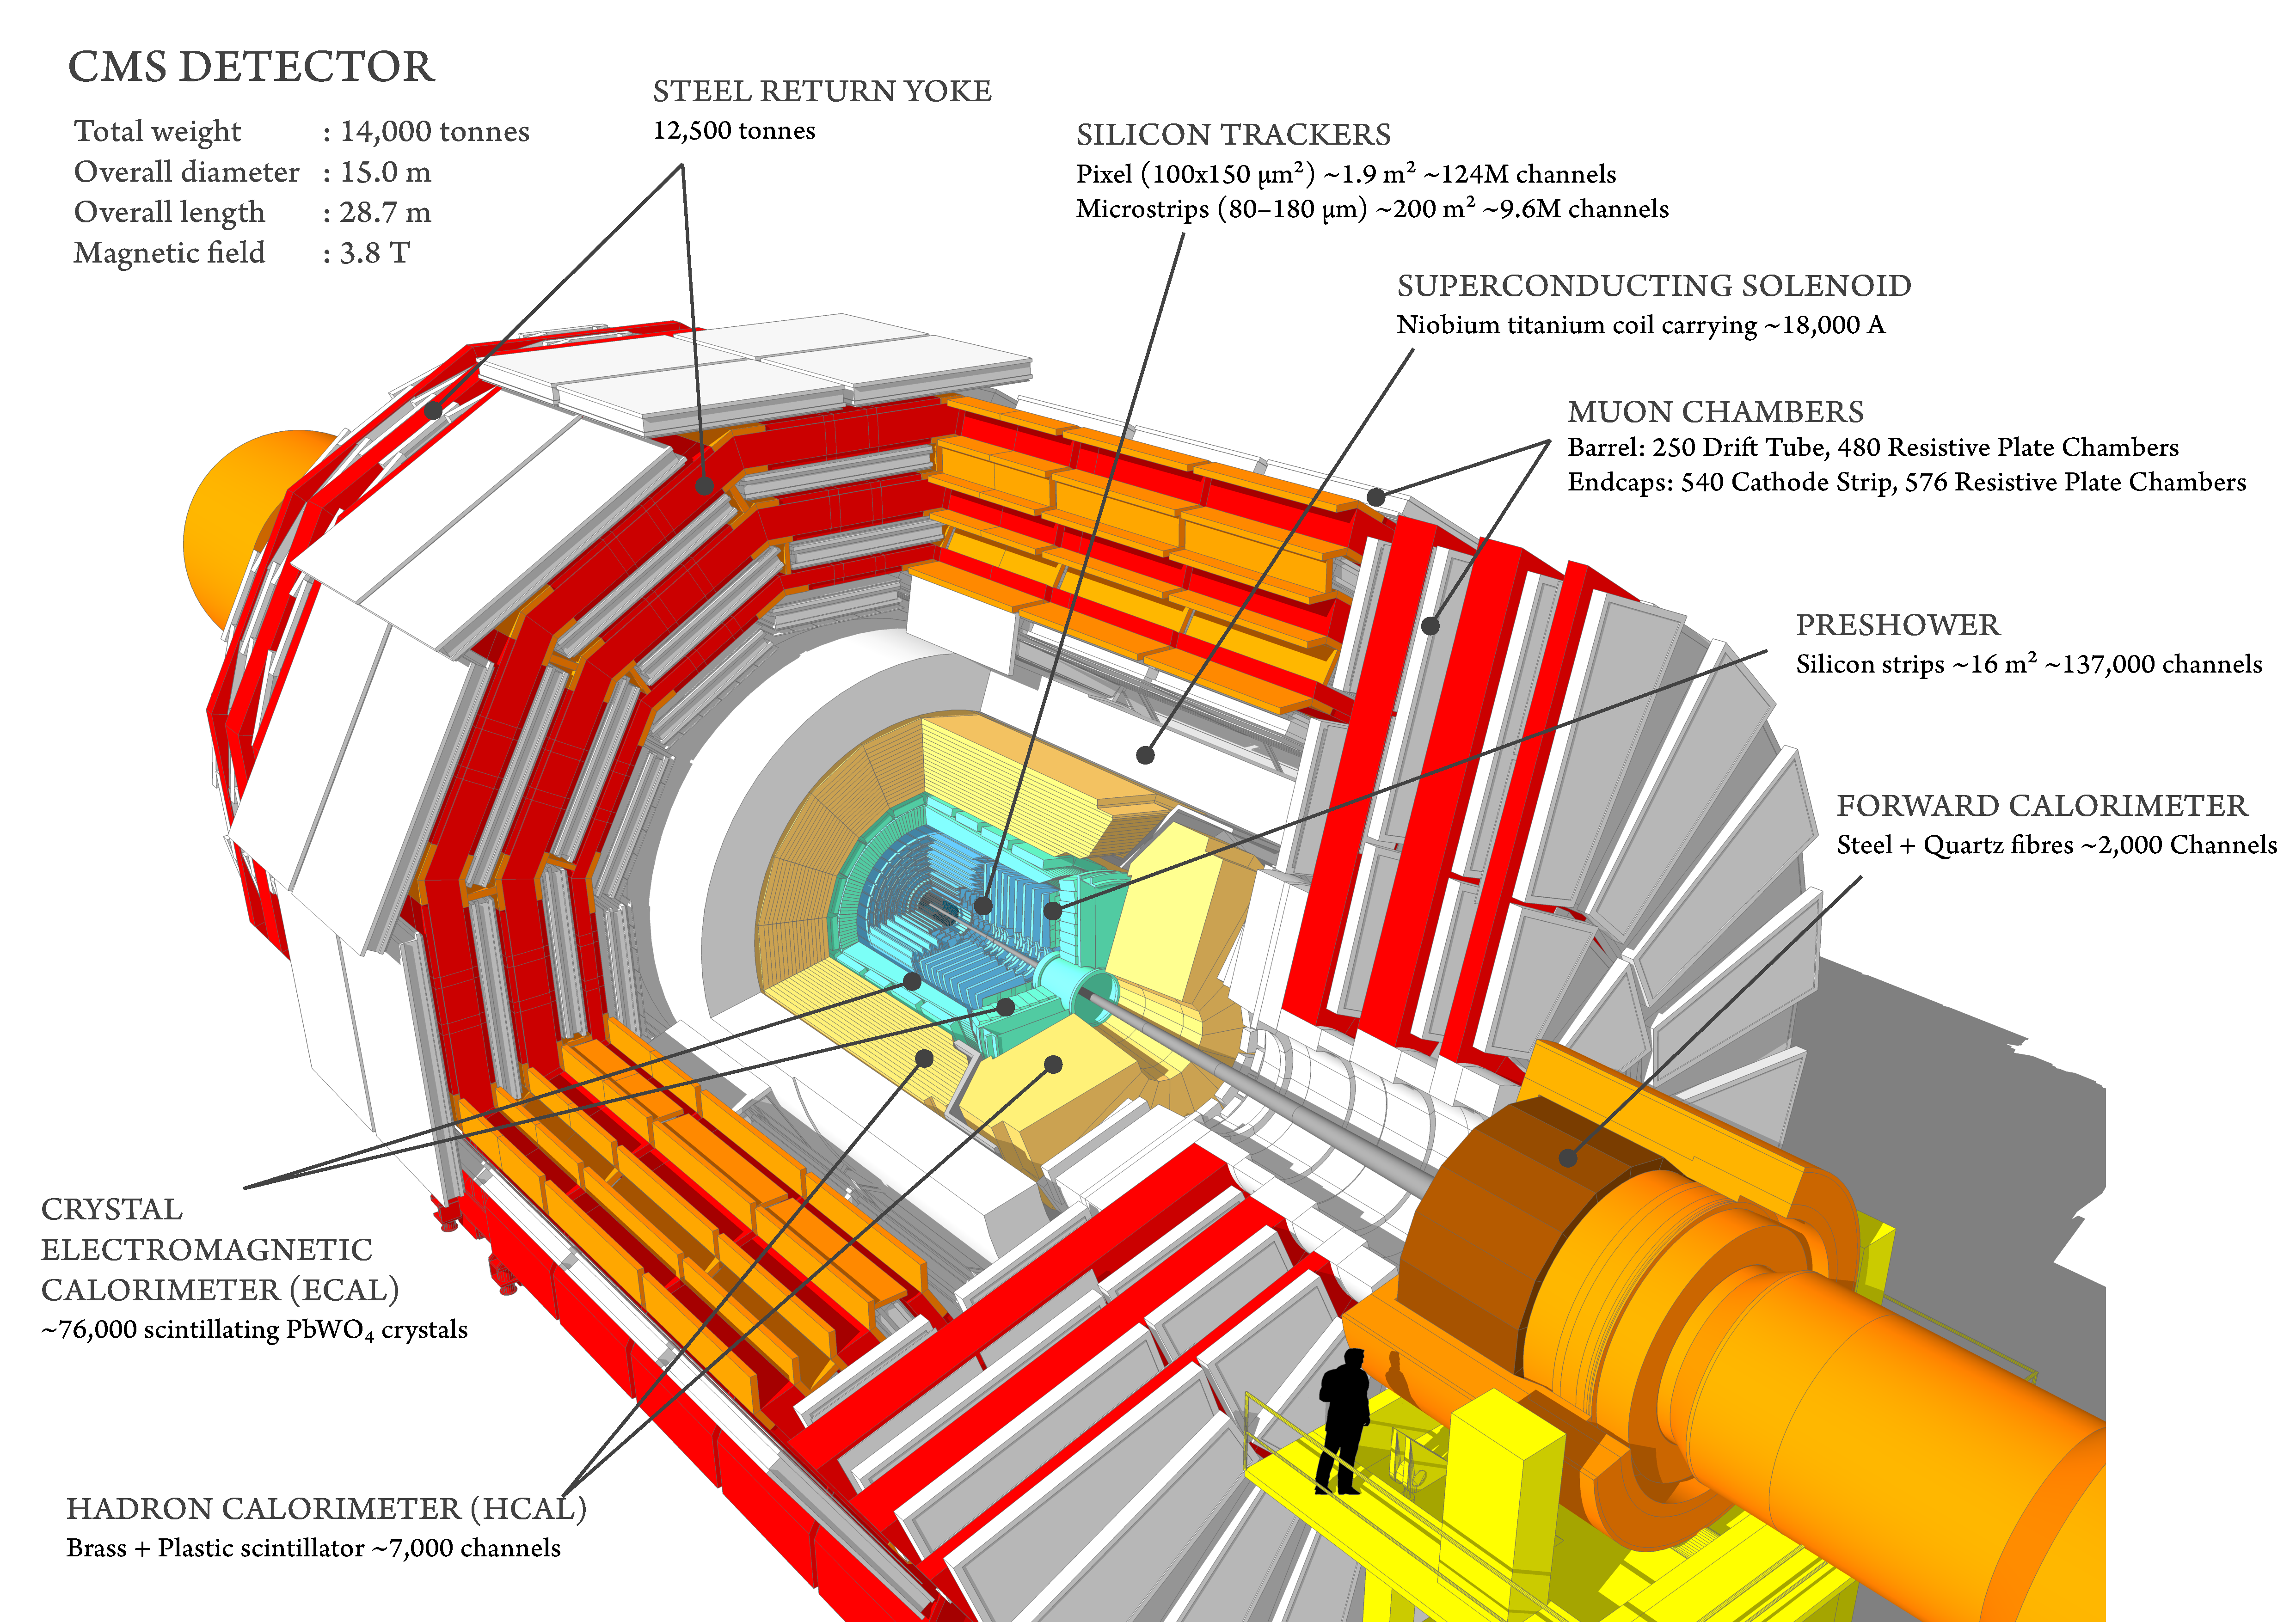
\includegraphics[width=\textwidth]{figures/cms_cutway_ME4_2.pdf}
  \caption[The CMS detector cutaway view]%
  {The CMS detector cutaway view~\cite{image-cms-cutway}}%
  \label{fig:cms-cutaway}
\end{figure}

The slice view of \gls{CMS} in Figure~\ref{fig:cms-slice}
shows how different particles leave signature in \gls{CMS} detector.
Neutral particles such photons, neutrinos, and hadrons will leave no track
in \gls{ST}, and are identified by only energy deposited or missing energy.
Electrons are identified from the track in \gls{ST} and energy deposit
in \gls{ECAL}, hadrons are heavier and they pass through \gls{ECAL}
and deposit their energy completely in \gls{HCAL}, leaving only small fraction
of energy in \gls{ECAL}.
Since muons are \gls{MIP}, they pass through whole detector with very small
fraction of energy deposit in \gls{ECAL} and \gls{HCAL}.

This section describes the subsystems of \gls{CMS} detector.
For detailed technical description refer to~\cite{CMS-JINST-S08004}.

\begin{figure}[!ht]
  \centering
  \includegraphics[width=\textwidth]{figures/cms_slice.png}
  \caption[The CMS detector slice view]%
  {The CMS detector slice view~\cite{image-cms-slice}}%
  \label{fig:cms-slice}
\end{figure}

\subsection{
  The CMS Coordinate System
}\label{ch_cms:cms-coordinate}

CMS uses \gls{IP} of collisions as origin to define right-handed
coordinate system. The \( z \)-axis is along the beamline,
the \( x \)-axis points toward the center of the \gls{LHC},
and the \( y \)-axis points upwards, toward Earth's surface.
The transverse plane \( x - y \) is used as to calculate
most commonly used quantities like transverse momentum \( p_{T} \)
and energy \( E_{T} \).

To describe the direction of particles leaving the \gls{IP},
azimuthal \( \phi \) and polar \( \theta \) angles are used.
\( \phi \) is measured around the beam axis,
and \( \theta \) is measured from the beam axis.
In collider physics, pseudorapidity \( \eta \) (Lorentz invariant) is used
to describe direction from beam pipe instead of \( \theta \) as,
%
\begin{equation}
  \eta = - \ln[\tan{\theta/2}]
\end{equation}

and sometimes in terms of rapidity \( y \) as,
%
\begin{equation}
  y = \frac{1}{2} \ln{\frac{E+p_{z}}{E-p_{z}}}
\end{equation}

Particles kinematics can be completely described in terms of
\( p_{T} \), \( \eta \), \( \phi \), and \( E_{T} \) or mass.
The distance between the two particles \( \Delta R \) in \( \eta - \phi \) plane
is described as,
%
\begin{equation}
  \Delta R = \sqrt{ {(\Delta \eta)}^{2} + {(\Delta \phi)}^{2} }
\end{equation}

\subsection{
  The Superconducting Magnet
}

The superconducting magnet is the main part of the \gls{CMS} detector, it is
12.5 meters long and 6.3 meters in diameter. The magnet is cooled to
4.5\,\text{K}\xspace and 20\,\text{kA}\xspace current flows through it to
generate 3.8\Tesla{} of magnetic field with stored energy of 2.6\,\text{GJ}\xspace.

The Figure~\ref{fig:cms-magnet} shows visible superconducting magnet
and iron yoke when part of \gls{CMS} detector was lowered in the underground
cavern during installation in 2007.

The key purpose of magnet is to determine the momentum and the sign of charged
particles by bending them. The momentum resolution of the particles will
decrease with increase in \(p_T \), with constant 3.8\Tesla{} magnetic field
inside and it has momentum resolution of \(\Delta p /p \approx 10 \% \), which
is enough to determine unambiguously the sign of muons with
momentum of \(\approx 1\TeV{}/c \).

\begin{figure}[!ht]
  \centering
  \includegraphics[width=0.75\textwidth]{figures/cms_magnet_lowered.jpg}
  \caption%
  [The picture of the CMS detector central part when lowered in underground
    cavern with superconducting magnet and iron
    yoke visible]%
  {The picture of the CMS detector central part when lowered in underground
    cavern with superconducting magnet and iron
    yoke visible~\cite{image-cms-magnet}.}%
  \label{fig:cms-magnet}
\end{figure}


\subsection{
  The Tracking System
}

The \gls{CMS} tracking system \gls{ST} is the innermost part of the detector, it
is made up of pixel and strip detectors. The main goal of \gls{ST} is to
reconstruct the tracks of the charged particles with high precision in high pileup
environment.

Silicon is most commonly used material for making tracking systems because of it's
semiconductor properties, and high radiation hardness which is essential for the
innermost detector. When a p-n junction is built on silicon substrate it creates
a depletion zone with no charge carriers at the junction, and whenever
a charged particle pass through the depletion zone it creates a electron-hole pair,
and under reverse bias this electron-hole generates electrical signal. The \gls{CMS}
tracking consists of about 124 million channels of such junctions in
pixel detector and 10 million in strip detector.

The pixel detector was upgraded in 2017 and the comparison of layers before
and after the upgrade is shown in Figure~\ref{fig:cms-pixel}. It is made up of
four barrel layers and three endcaps, with nearest barrel layer being 3\cm{}
away from beamline for precise measurement of \gls{IP}.
Because of the large number of pixel channels, the readout is done by \glspl{ASIC}.

\begin{figure}[!ht]
  \centering
  \begin{minipage}[c]{.62\textwidth}
    \includegraphics[trim={80pt 0 80pt 0},clip,width=\textwidth]%
    {figures/cms_pixel_phase1.pdf}
  \end{minipage}
  \begin{minipage}[c]{.35\textwidth}
    \includegraphics[width=\textwidth]{figures/cms_pixel_phase1_04.png}
  \end{minipage}
  \caption[The CMS pixel upgrade]%
  {The CMS pixel upgrade. The left is cross sectional view of pixel detector
    layers before upgrade (bottom) and after Phase 1 upgrade (top).
    The right is view pixel barrel before upgrade (left)
    and after upgrade (right)~\cite{image-cms-pixel}.}%
  \label{fig:cms-pixel}
\end{figure}

The outermost part of \gls{ST} detector is made of silicon strips. It allows large
coverage by reducing number of readout channels. It has 10 layers in barrel region
and 12 discs in endcap region. For better signal-to-noise ratio and radiation
tolerance both pixel and strip operates at -20\,\de\text{C}\xspace.

\subsection{
  The Electromagnetic Calorimeter
}

The \gls{ECAL} active material is made of lead tungstate (PbWO\textsubscript{4})
scintillating crystals and two layers silicon strip for preshower
in front of the endcaps. The crystals in central barrel section are mounted
in quasi-projective geometry pointing towards \gls{IP} and covers
\( |\eta| < 1.48 \), and two endcaps extends the coverage to
\( |\eta| = 3.0 \). The schematic layout of \gls{ECAL} is shown in Figure~\ref{fig:cms-ecal-schematic}
and the picture of endcap quadrant when assembled in Figure~\ref{fig:cms-ecal-ee}

The main purpose of \gls{ECAL} is to determine energy and positions of
electromagnetically interacting particles. To determine particle need to completely
deposit their energy, except electron and photons all other particles pass
through \gls{ECAL} crystals with only small fraction of energy signature in crystals.
When electron and photon interacts with PbWO\textsubscript{4} it starts the process
of electromagnetic shower and continues until the energy the energy of the incident
particle is below threshold, which is about 1\MeV{}.

\begin{figure}[!ht]
  \centering
  \begin{minipage}[c]{.60\textwidth}
    \includegraphics[width=\textwidth]{figures/cms_ecal_schematic.pdf}
  \end{minipage}
  \begin{minipage}[c]{.38\textwidth}
    \includegraphics[width=\textwidth]{figures/cms_ecal_layout.png}
  \end{minipage}
  \caption[The CMS \gls{ECAL} schematic layout]%
  {The \gls{CMS} \gls{ECAL} schematic layout. The left is schematic showing arrangement of
    superclusters in barrel and endcap (with preshower layers). The right is \(y-z \)
    plane quarter view of \gls{ECAL} layout~\cite{image-cms-ecal-layout}.}%
  \label{fig:cms-ecal-schematic}
\end{figure}

The resolution of the \gls{ECAL} energy measurements can be described as,
%
\begin{equation}
  {\left( \frac{\sigma}{E} \right)}^2
  = {\left( \frac{S}{\sqrt{E}} \right)}^2
  + {\left( \frac{N}{E} \right)}^2
  + C^2
\end{equation}

where \(S \) is the stochastic term, \(N \) is related to the noise,
and C is a constant offset.

\begin{figure}[!ht]
  \centering
  \includegraphics[width=0.60\textwidth]{figures/cms_ecal_ee_quadrant.jpg}
  \caption[The \gls{ECAL} endcap quadrant assembled view]%
  {The \gls{ECAL} endcap quadrant assembled view~\cite{image-cms-ecal-ee-quadrant}.}%
  \label{fig:cms-ecal-ee}
\end{figure}

\subsection{
  The Hadronic Calorimeter
}

\gls{HCAL} is last subdetector inside solenoid after
\gls{ECAL} and the first half of barrel \gls{HCAL} inserted is shown in
Figure~\ref{fig:cms-hcal-inserted}. Similar to \gls{ECAL} the purpose of \gls{HCAL}
is to shower hadrons, and measure their energy and position. \gls{HCAL} is made up of
towers pointing towards \gls{IP} and each tower is made up of sampling layers
with alternating layers of plastic scintillator and brass.
Brass acts as absorber in \gls{HCAL} and causes hadrons to shower, then from the light
output of scintillator receiving secondary shower particles gives the amount of
energy deposit in each layer. In phase 1 upgrade the \gls{HCAL} was upgraded
to give energy deposit as function of depths and the depth segmentation schematic is
show in Figure~\ref{fig:cms-hcal-depth} and the details of upgrade are in technical design
report~\cite{cms-hcal-upgrade}.

\begin{figure}[!ht]
  \centering
  \includegraphics[width=\textwidth]{figures/cms_hcal_hb_inserted.jpg}
  \caption[The first half of the barrel \gls{HCAL} inserted into the
    superconducting solenoid (April 2006)]%
  {The first half of the barrel \gls{HCAL} inserted into the
    superconducting solenoid (April 2006)~\cite{image-cms-hcal-inserted}.}%
  \label{fig:cms-hcal-inserted}
\end{figure}

\gls{HCAL} consists barrel (HB) and two endcaps (HE) located inside solenoid.
These two subsystems combined cover region \( |\eta| = 3.0 \), which
is most of physics analysis done in \gls{CMS}.
There are two another subsystems of \gls{HCAL} outside solenoid,
a forward \gls{HCAL} (HF) and outer barrel \gls{HCAL} (HO).
HO was added to ensure there is no leak from the particles that
make past the solenoid. HF extends the coverage
to \(|\eta| = 5.0\) and is based Cherenkov radiation principle unlike
other subsystems of \gls{HCAL}, and it uses quartz fiber
as active material with steel absorbers.
HF is used most commonly used by heavy ion analysis.

\begin{figure}[!ht]
  \centering
  \includegraphics[width=\textwidth]{figures/cms_hcal_depth_seg.pdf}
  \caption[The \gls{HCAL} depth segmentation after phase 1 upgrade]%
  {The \gls{HCAL} depth segmentation after phase 1 upgrade~\cite{image-cms-hcal-depth}.}%
  \label{fig:cms-hcal-depth}
\end{figure}

\subsection{
  Muon Detector
}

The outermost subsystem in the \gls{CMS} detector is the muon detector.
Unlike electrons, muons are \glspl{MIP}, they do not lose much of their energy
while passing through tracker, calorimeter and solenoid.
Muon detector is build to identify, measure momentum and trigger the events
with muons. Like other subsystems, muon detector consists of barrel and endcap
detector and schematic layout is highlighted in Figure~\ref{fig:cms-muon-system}.

The muon detector consists of three subsystems \glspl{DT}, \glspl{CSC} and
\glspl{RPC}.

The \glspl{DT} are wire gas detectors filled with Argon and composed of
many tube cells of about 4\cm{}. Muon passing through these tubes
ionizes Argon and free electron is detected with wires as cathode.
Each DT is about 2 meters by 2.5 meters in size, and there are four layers
of the \glspl{DT} interleaved with iron yoke parallel to
the beam pipe in barrel region. The drift time is the order of about 380\nanoseconds.

\begin{figure}[!ht]
  \centering
  \includegraphics[width=0.9\textwidth]{figures/cms_muon_system.pdf}
  \caption[The quadrant view of CMS subdetectors layout, and
    the coverage of the muon detector \glspl{DT}, \glspl{CSC},
    and \glspl{RPC} highlighted]%
  {The quadrant view of CMS subdetectors layout, and
    the coverage of the muon detector \glspl{DT}, \glspl{CSC},
    and \glspl{RPC} highlighted~\cite{image-cms-muon-system}.}%
  \label{fig:cms-muon-system}
\end{figure}

The \glspl{CSC} are based on same principle as \glspl{DT},
and are made of multi-wire proportional chambers consisting of
6 anode planes interleaved with 7 cathode planes. They have time resolution
smaller than 5\nanoseconds. The \glspl{CSC} are used in endcap region,
where radiation hardness is required, and non uniform magnetic field does neutrinos
effects the the measurement.

The \glspl{RPC} are made up of two high resistive parallel
plates, with oppositely charged plates and gas volume between them.
When a charged particles passes through it and ionizes the gas, it creates
an avalanche and charge is collected by metallic readout strips.
\glspl{RPC} have poor position resolution but fast readout of the order of 1\nanoseconds,
which is fast compared to \glspl{DT}, this is the reason there are 1 or 2 \glspl{RPC}
attached to both \glspl{DT}, and \glspl{CSC}.

\subsection{
  Level 1 Trigger
}

Since proton-proton collisions happens every bunch crossing which is
25\nanoseconds{} apart, which is equivalent to 40\,\text{MHz}\xspace collisions rate.
At this collisions rate, the data storage required will be enormous
and \gls{CMS} can only record up to 1000 events per second. Since most of events
does not contain interesting physics events, they can be thrown away.
To do this \gls{CMS} has two tier trigger system \gls{L1T}, and \gls{HLT}.

The \gls{L1T} is the foremost electronic processing system through
which event information is processed before it is passed to
second trigger system \gls{HLT}.
The \gls{L1T} is designed to make fast decisions in about 3.8\mus,
and only uses \gls{ECAL}, \gls{HCAL} and muon system to make decision.
\gls{L1T} cut downs the data rate from 40\,\text{MHz}\xspace to
100\,\text{kHz}\xspace. The \gls{L1T} electronics is placed next to
the detector in underground cavern for fast transfer of data.

The \gls{HLT} further reduces the data rate from 100\,\text{kHz}\xspace to
about 1\,\text{kHz}\xspace using a computer farm with nearly 26000 cores.
\gls{HLT} uses all the available information from the event to make
decision in about 300m\seconds. \gls{HLT} is modular by design
to allow the use of information from different systems to construct
multiple paths called \gls{HLT} paths, for example the single muon \gls{HLT}
path will save event with at least one muon passing the selection criteria
set in \gls{HLT} path. Events passing at least on \gls{HLT} path are
save for offline physics analysis.

\chapter{
  Event Simulation and Reconstruction
 }\label{ch_reco}

The proton-proton collision at \gls{LHC} produces shower of particles, before
the event information can be easily used in an analysis, the data collected goes
through iterative process of reconstruct particles produced in collision.
\gls{CMS} uses \gls{PF} algorithm to reconstruct 4-vectors of muons, electrons,
photons, hadrons, jets and missing transverse momentum~\cite{cms-particle-flow-2017}.

To analyze the data collected and compare it with theoretical model, events are
simulated using \gls{MC} event generators and are passed through detector simulation
and \gls{PF} so that \gls{MC} events can be treated same as real events.

This chapter describes the basic ingredients for object reconstruction, \gls{PF}
candidates and \gls{MC} event generators used in this analysis.

\section{
  Track Reconstruction and Calorimeter Clustering
 }\label{ch_reco:track-calo}

For complete particle reconstruction two main ingredients are tracks left by particle
in the detector, and energy deposit in calorimeter. This section describes track reconstruction
from the hits in Tracker and Muon Detector, and energy deposit measurement from
calorimeter clustering.

Track reconstruction requires reconstructed hits, and seed generation which are
described in~\cite{cms-track-vertex}, then the track reconstruction is done using
pattern recognition which is based on combinatorial \gls{KF} method~\cite{cms-track-reco}.
It is an iterative process starting from seed layer the track is estimated and then
proceeds to next layer one by one, at each successive layer the track trajectory
is better known. There can be multiple hits in each new layer, for this multiple
trajectory candidates are created. All the trajectory candidates are grown in parallel
to avoid bias, and truncated at each layer to prevent exponential increase
in number of candidates. Then finally the track is fitted to compute momentum
and vertex information.

The main purpose of calorimeter clustering is to determine position and
energy deposit of the particle. A cluster in a calorimeter is a local group of
energy deposits that are spatially consistent with a electromagnetic
or hadronic shower. First the topological
clusters are identified, a topological cluster is a contiguous region of energy
deposit, then a seed is identified in topological cluster with certain energy
threshold, and highest among the 8 neighbors for \gls{ECAL} and 4 neighbors for \gls{HCAL}.
Now starting with seed energy and position, the neighbors energy are added, and
new position is calculated. For the case when we have just one seed, there is only
iteration until all the neighbors are added, in case when we have more than one seeds
in a cluster, the energy from neighbors is shared, the fraction of energy shared
depends on the energy and position of the cluster, after the first
iteration of calculation of the energy and position the
process is repeated with new values of cluster's energy and
position until either the maximum iteration is reached or cluster's energy and position
values are converged.

\section{
  Reconstructed Particles
 }

After tracks and calorimeter clusters are formed, \gls{PF} links this information
from the detectors together to form objects as broadly discussed in
Section~\ref{ch_cms:cms} and shown in Figure~\ref{fig:cms-slice}. This section
describes the properties of those reconstructed particle candidates.

\subsection{
  Muons
}

Reconstructing muon with best precision is the key ingredient for many physics
searches. Muons reconstruction and identification uses all the information from tracker,
calorimeters and muon detector. There are two types of reconstruction performed
``Global'' and ``Tracker'' for muon candidates. Global muons are formed combining and refitting
muon hits in the muon detector with compatible track from \gls{ST}, and the tracker muons
are formed by extrapolating tracks from \gls{ST} to segments in muon detector.

Once the muon candidates are found, the kinematics properties (\( p_T, \eta, \phi \))
are calculated from track fitting, and other properties such as distance form
\gls{PV} \( dxy \), \( dz \), number of hits in the tracker and muon system, tracker
based relative isolation (\ref{eq:trackerRelIso-muon}) in a cone of \( \Delta R = 0.3 \), and
\gls{PF} relative based isolation (\ref{eq:pfRelIso-muon})
in a cone of \( \Delta R = 0.4 \) are stored for cleaning and isolating muons for
physics analysis.

The tracker and \gls{PF} based relative isolation are defined as,
%
\begin{equation}\label{eq:trackerRelIso-muon}
  \text{TkIso03} = \left( \sum p_{T}^{\text{Tracks (PV)}} \right) /
  \left( p_{T}^{\mu} \right)
\end{equation}
%
\begin{equation}\label{eq:pfRelIso-muon}
  \text{PFRelIso04} = \left( \sum p_{T}^{\text{CH (PV)}}
  + \min \left[ 0, \sum E_{T}^{\text{NH}} + \sum E_{T}^{\gamma}
    - 0.5 \sum p_{T}^{\text{CH (PU)}} \right] \right) /
  \left( p_{T}^{\mu} \right)
\end{equation}

where ``Tracks (PV)'' refers to all the tracks in tracker and coming from \gls{PV},
``CH (PV)'' and ``CH (PU)'' refers to charged hadrons coming from \gls{PV} and \gls{PU}
respectively, ``NH'' refers to neutral hadrons, \( \mu \) refers to muon, and
\( \gamma \) refers to photon.

There are multiple source of muons whenever collision event happens, they can be
real muons or hadrons which are misidentified as muons, these hadrons
are able ``punch'' through \gls{HCAL} and leaves hit in muon detector. The real
muons of interest are called ``prompt'' muons and others are either usually referred
as ``fake'' or ``non-prompt''. Fake muons can originate from decay of pions and kaons in flight
usually identified with a ``kink'' in track or from heavy flavor decay of b or c-quarks
which are identified with tracks not originating form \gls{PV}.
The prompt muons are the ones coming from decay of H, W, Z bosons and \( \tau \) leptons,
and have small impact parameter from \gls{PV}, have hits in both tracker
and muon detector, and are typically well isolated.

In addition to muons from collision events, there can be cosmic muons from pion decay in
upper atmosphere. Cosmic muons are generally not in-time with collision and far from
interaction points.

\subsection{
  Electrons and Photons
}

Since there is large amount of material in tracker, electrons often emit bremsstrahlung
photons when passing through tracker volume,
and photons can further decay to \( e^- e^+ \) pair which complicates the
tracking algorithm. The energy deposit of such electrons
emitting bremsstrahlung will have large spread in \( \phi \) direction because
the magnetic field will bend electrons in \( \phi \) whereas photons are unaffected.
For this reason electron and photon reconstruction are done together, and
the \gls{GSF} algorithm is used for electron track reconstruction
which takes care of kinks in electrons track because of hard emission~\cite{cms-electron-gsf}.

An electron is reconstructed when an \gls{ECAL} cluster matches a \gls{GSF} track,
and a photon is reconstructed when an \gls{ECAL} cluster with \( E_T \)
more than 10\GeV{} is found and have no matching \gls{GSF} track. To prevent
electron and photon from being misidentified as jets certain conditions are applied,
for electron the number of \gls{GSF} track matching with \gls{ECAL} cluster is limited to
maximum of two, and energy deposit in a cone of \( \Delta R = 0.15 \) in \gls{HCAL}
around the position of electrons and photons is required to be less than 10\%.

Similar to muons, after electron and photon reconstruction is done, their kinematics properties
are calculated and various other properties required for cut based
and \gls{MVA} based identification are stored. The detailed description of electrons
and photons identification technique and properties used in this dissertation
can be found in Reference~\cite{cms-egamma-id}.

\subsection{
  Hadrons and Jets
}

Quarks and gluons produced in a collision event are not detected directly,
because of color confinement, they go through fragmentation and
hadronization making a collimated spray of particles mostly made of hadrons
and are called ``jets''. Charged hadrons are reconstructed when a \gls{HCAL} cluster can be associated with
one or more tracks, if the track association fails the cluster is reconstructed as
neutral hadron.

Jet in \gls{CMS} are reconstructed using \FASTJET{} package~\cite{fastjet-manual},
which takes input of all \gls{PF} candidates and associated tracks. The clustering
basically combines 4-vectors of particles iteratively and stop when distance between
two particles (\( d_{ij} \)) is higher than stopping distance (\( d_{iB} \)).

\( d_{ij} \) and \( d_{iB} \) are defined as,
%
\begin{equation}
  d_{ij} = \min (p_{Ti}^{2p}, p_{Tj}^{2p}) \frac{\Delta R_{ij}^{2}}{R^{2}}
\end{equation}
%
\begin{equation}
  d_{iB} = p_{Ti}^{2p}
\end{equation}

where \( p \) is the parameter for different clustering algorithms, \( R \) is the
cone size, and
\( \Delta R_{ij} \) is distance between two particles in iteration.

Anti-\( k_T \) (AK) is the most use jet algorithm in physics analysis, this corresponds to
\( p = -1\), this means the hard particles will be clustered first in this clustering
algorithm.
The cone size used for standard jets (AK4) is \( R = 0.4 \), and for large jets (AK8) often called
``fatjet'' is \( R = 0.8 \).

To mitigate the effect of \gls{PU} contamination in jets two most commonly used
techniques are \gls{CHS} and \gls{PUPPI}~\cite{puppi2014}.
\gls{CHS} as the name suggests removes all the \gls{PF} in the jet clustering which are
originating from \gls{PU} vertices, and it is a standard technique for AK4 jets.
\gls{PUPPI} works by identifying \gls{PU} in an event from charged \gls{PU} information,
then it assigns a weight to all the other particles inside jet, such as neutral particles,
the weight is then used to rescale momentum of those particles.
The main limitation of \gls{CHS} is that it only removes charged \gls{PU} contribution,
for larger jets it can be issue, since it is clustering larger number of particles
and can have significant contribution from neutral hadrons, for this reason \gls{PUPPI}
technique is used for AK8 jets.

To improve the jet selection and reject jets originating purely from \gls{PU}
two methods are used in this dissertation, jet identification based on
multiplicities and energy fraction of particles contained in the jet,
and \gls{MVA} based \gls{PU} identification which uses jets shape
variables to discriminate prompt jet from pileup jets.
The details of \gls{PU} mitigation and identification used in
\gls{CMS} are described in Reference~\cite{cms-jme-pu-run2}.

After jets reconstruction is complete the in addition to calculating kinematics
properties (\( p_T \), \( \eta \), \( \phi \) and mass), various other
properties such as b-quark tagging and quark-gluon likelihood are also
calculated and stored.

\subsubsection{
  N-Subjetiness and Deep Taggers
}

The origin of fatjets are usually when heavy energetic particle
often referred to as ``boosted'' decays hadronically,
for example boosted W or Z bosons decaying to a pair of quarks.
To find and discriminate the fatjet of interest based on in it's substructure
the two technique studied and used are N-Subjetiness~\cite{tau21-paper}
and ``deep tagger''~\cite{cms-jme-deep-tagger}.

N-Subjetiness is defined as,
%
\begin{equation}
  \tau_N = \frac{1}{d_0} \sum_k p_{T,k} \min \{ \Delta R_{1,k}, \Delta R_{2,k}, \ldots , \Delta R_{N,k} \}
\end{equation}

where \( k \) runs over constituent particles in a jet, \( \Delta R_{J,k} \)
is the distance between subjet \( J \) and \( k \) constituent, and \( d_0 \)
is the normalization constant defined as,
%
\begin{equation}
  d_0 = \sum_k p_{T,k} R_0
\end{equation}

\( \tau_N \) quantifies to what degree a jet can be regarded as made of \( N \) jets.
The small values of the \( \tau_N \) means a jet is more likely to have
\( N \) or less subjets, and higher value means it will at least have \( N + 1\)
subjets. Rather than using \( \tau_N \) alone, ratio of different \( \tau_N \)
variables is used, which more discriminating for cases like W vs QCD jets.
Figure~\ref{fig:cms-tau21-tau32-comparison} shows distribution of
\( \tau_{21} \) and \( \tau_{32} \) shapes in signal and background.
\( \tau_{21} \) is used to discriminate fatjets with 2-prongs (W/Z/H)
and \( \tau_{32} \) with 3-prongs (t-quark) substructure against QCD jets.

\begin{figure}[!ht]
  \centering
  \includegraphics[width=\textwidth]{figures/CMS_JME_18_002_Figure_003.pdf}
  \caption[Comparison of \( \tau_{21} \) and \( \tau_{32} \) shapes for signal and background in AK8 jets]%
  {Comparison of \( \tau_{21} \) and \( \tau_{32} \) shapes for signal and background in AK8 jets.
    The left is \( \tau_{21} \) distribution showing discrimination W/Z/H jets
    vs QCD jet, and the right is \( \tau_{32} \) distribution for t-quark vs
    QCD jets~\cite{cms-jme-deep-tagger}.}%
  \label{fig:cms-tau21-tau32-comparison}
\end{figure}

Deep Tagger for AK8 are \gls{ML} based tagger developed to determine
origin of a fatjet. These taggers are trained on particle level information
from \gls{PF} and provide multi class tagging probabilities. In addition to
there are version of these taggers is also which is de-correlated from the mass of jet,
this is important for analysis including this dissertation where we utilize
mass regions of fatjet to normalize background contribution. Figure~\ref{fig:cms-deepAK8-arch}
describes the architecture of ``DeepAK8'' tagging.

\begin{figure}[!ht]
  \centering
  \includegraphics[width=0.9\textwidth]{figures/CMS_JME_18_002_Figure_009.pdf}
  \caption[The network architecture of DeepAK8]%
  {The network architecture of DeepAK8~\cite{cms-jme-deep-tagger}}%
  \label{fig:cms-deepAK8-arch}
\end{figure}

\subsubsection{
  Softdrop Mass
}

Fatjets can also have contamination coming from wide angle
soft \gls{ISR} and multiple hadron scattering,
which affects the mass calculation of the jet, to remove
such contamination and have better mass reconstruction, the
``softdrop'' mass algorithm~\cite{softdrop-mass-2014} is used.

Softdrop is a declusttering algorithm which removes the particle from the jet
with radius \( R_0 \), when the following condition between two particles is satisfied,
%
\begin{equation}
  \frac{\min(p_{T,1}, p_{T,2})}{p_{T,1} + p_{T,2}} > z_{cut} {\left( \frac{\Delta R_{12}}{R_0} \right)}^{\beta}
\end{equation}

where \( \Delta R_{12} \) is the distance between the two particles, \( z_{cut} \)
and \( \beta \) are the parameters for tuning softdrop declusttering.
For fatjets used in \gls{CMS}, they have softdrop applied with
\( \beta = 0\) and \( z_{cut} = 0.1\) which vetoes both soft
and soft-collinear emissions in a jet.

\subsection{
  Missing transverse momentum
}

Invisible particles like neutrinos cannot be detected at \gls{CMS} directly.
Kinematics of such particles can be determined using laws of conservation of
total momentum. In case of proton-proton collision,
the actual collision happens between quarks contained in
proton and quarks carry fraction of proton momentum
and can not be determined exactly, for this reasons kinematic determination
of invisible particles is limited to transverse plane only.

After all the particles are reconstructed in an event, their \( p_T \)'s
can be used to determine missing transverse momentum as,
%
\begin{equation}
  \vec{p}_{T}^{~miss} = - \sum \vec{p}_{T}
\end{equation}

It's usually neutrinos which contributes to missing transverse momentum,
and they have very small mass, the missing transverse momentum is then
equivalent to \gls{MET}, which is most often used term in physics analysis.

\section{
  Monte Carlo Simulation
 }

\subsection{
  Generators
}

\subsection{
  Hadronization
}

\chapter{
  VBS Measurement in ZVjj Final State
 }\label{ch_vbs}

As discussed in Section~\ref{ch_intro:vbs} this analysis targets
\gls{VBS} of ZV with two jets in final state. The goal of the analysis
is to reduce contribution from background processes as much as possible
without loosing much of signal, and measure signal strength and significance.

Since Z decays leptonically and V is decaying hadronically,
the phase-space of this analysis can be either
\( l^+ l^- jjjj \) or \( l^+ l^- J jj\), where \( l \) are leptons,
\( j \) are narrow jets and \( J \) is a boosted (wider) jet.
The phase-space is divided into two broad regions signal and controlled,
signal region is constructed based on theory such that it is mostly signal process
and controlled region is basically orthogonal to the signal region
where we expect contributions mostly from background processes.

The analysis is performed ``blind'' to avoid intrinsic bias
i.e.\ until the analysis procedure is finalized, the collision data is only used
in controlled regions. Once the analysis technique is optimized using \gls{MC}
samples and validated against collision data in controlled regions. Once the
analysis technique is satisfactory and approved by \gls{CMS} Physics Group
then the results are ``un-blinded'' i.e.\ measurements are done
using collision data in signal region.

\section{
  Dataset and Simulation
 }

As discussed in Section~\ref{ch_cms:L1T} only events those pass Level-1
Trigger and \gls{HLT} paths are saved for further processing, \gls{MC}
simulation also have these identical step during event generation to mimic
Level-1 Trigger and \gls{HLT} paths.

\gls{CMS} collaboration processes the datasets centrally and provides various
tiers of datasets such as ``RECO'' datasets, which contains reconstructed
objects and no skimming. Average size of an event saved at ``RECO'' tier is
480 kB per event and on average an analysis will process
3 billion events, which makes this tier not practical in terms of computer processing
time and storage if each analysis starts from ``RECO''. \gls{CMS} centrally
processes these datasets further and removes certain objects
or features to reduce the average event size but still covering
majority of the analysis to make use of the reduced datasets.

This analysis uses \NanoAOD{} tier with version ``v7'' of datasets
which has average event size of 2--3 kB.

\subsection{
  Data
}

The collision data events used in this analysis are all certified
by \gls{CMS} \gls{DQM} and \gls{DC} group. The primary trigger object in
\gls{HLT} paths are leptons \( p_{T} \) threshold, and since in our final state
we are looking for Z boson decaying into two leptons, we require single and
double lepton trigger for our analysis. Depending on the detector
conditions and \gls{LHC} storage capacity we have slightly different threshold
in triggers across different years. The Table~\ref{tab:hlt-paths} contains the list of
\gls{HLT} paths used in this analysis.

\begin{table}[!ht]
  \centering
  \caption{Trigger paths used to select events in CMS collision data}
  \begin{tabular}{cll}%
    \toprule
    Dataset & Year                  & HLT Path                                          \\
    \midrule
    \multirow{4}{*}{Single Muon}
            & \multirow{2}{*}{2016} & \url{HLT_IsoMu24}                                 \\
            &                       & \url{HLT_IsoTkMu24}                               \\
    \cmidrule(lr){2-3}
            & \multirow{1}{*}{2017} & \url{HLT_IsoMu27}                                 \\
    \cmidrule(lr){2-3}
            & \multirow{1}{*}{2018} & \url{HLT_IsoMu24}                                 \\
    \midrule
    \multirow{4}{*}{Single Electron}
            & \multirow{2}{*}{2016} & \url{HLT_Ele27_WPTight_Gsf}                       \\
            &                       & \url{HLT_Ele25_eta2p1_WPTight_Gsf}                \\
    \cmidrule(lr){2-3}
            & \multirow{1}{*}{2017} & \url{HLT_Ele35_WPTight_Gsf}                       \\
    \cmidrule(lr){2-3}
            & \multirow{1}{*}{2018} & \url{HLT_Ele32_WPTight_Gsf}                       \\
    \midrule
    \multirow{6}{*}{Double Muon}
            & \multirow{3}{*}{2016} & \url{HLT_Mu17_TrkIsoVVL_Mu8_TrkIsoVVL_DZ}         \\
            &                       & \url{HLT_Mu17_TrkIsoVVL_TkMu8_TrkIsoVVL_DZ}       \\
            &                       & \url{HLT_TkMu17_TrkIsoVVL_TkMu8_TrkIsoVVL_DZ}     \\
    \cmidrule(lr){2-3}
            & \multirow{2}{*}{2017} & \url{HLT_Mu17_TrkIsoVVL_Mu8_TrkIsoVVL_DZ_Mass8}   \\
            &                       & \url{HLT_Mu17_TrkIsoVVL_Mu8_TrkIsoVVL_DZ_Mass3p8} \\
    \cmidrule(lr){2-3}
            & \multirow{1}{*}{2018} & \url{HLT_Mu17_TrkIsoVVL_Mu8_TrkIsoVVL_DZ_Mass3p8} \\
    \midrule
    \multirow{4}{*}{Double Electron}
            & \multirow{2}{*}{2016} & \url{HLT_Ele23_Ele12_CaloIdL_TrackIdL_IsoVL_DZ}   \\
            &                       & \url{HLT_Ele23_Ele12_CaloIdL_TrackIdL_IsoVL}      \\
    \cmidrule(lr){2-3}
            & \multirow{1}{*}{2017} & \url{HLT_Ele23_Ele12_CaloIdL_TrackIdL_IsoVL}      \\
    \cmidrule(lr){2-3}
            & \multirow{1}{*}{2018} & \url{HLT_Ele23_Ele12_CaloIdL_TrackIdL_IsoVL}      \\
    \bottomrule
  \end{tabular}\label{tab:hlt-paths}
\end{table}

\subsection{
  MC Simulations
}

The \gls{EW} \gls{VBS} process which is our signal is
generated with \MADGRAPH{}5+\PYTHIA{}8 at \gls{LO} with \( \alpha_{EW}^{6} \) order
i.e.
all vertices in tree level Feynman diagram are \gls{EW} vertices.
The \gls{QCD} induced \gls{VBS} background process which is very
similar to our signal is generated with same configuration
but with \( \alpha_{EW}^{4} \alpha_{QCD}^{2} \) order i.e.
two of the six vertices are \gls{QCD}. The dominant background to analysis
\gls{DY} + Jets and, top-quark based processes consisting of
single top-quark (t and s-channel),
single top-quark in association with W boson (tW) and top-quark pair (t\=t) production.
The \gls{DY} + Jets are generated at \gls{LO} with \MADGRAPH{}5+\PYTHIA{}8
in bins of HT i.e.
scalar sum of all the jets \( p_{T} \) in the event, to have more statistics
for higher HT bins. Top-quark background process are generated at \gls{NNLO},
s-channel is generated with \MGvATNLO+\PYTHIA{}8 and others
t-channel, tW, t\=t are generated with \POWHEG{}+\PYTHIA{}8.
The complete list of Table~\ref{tab:mc-list-1},~\ref{tab:mc-list-2},~\ref{tab:mc-list-3} contains
the list of Signal and Background MC samples used for modeling in this analysis.

\begin{sidewaystable}[!ht]
  \centering
  \caption{List of MC samples for Signal and Background modeling}
  \resizebox{\textwidth}{!}{%
    \begin{tabular}{llll}%
      \toprule
      Process & Year       & Dataset Name                                                                      & Cross Section (pb) \\
      \midrule
      \midrule
      \multirow{6}{1.1in}{
        VBS\_EWK (Signal)}
              & 2016       & \url{WminusTo2JZTo2LJJ_EWK_LO_SM_MJJ100PTJ10_TuneCUETP8M1_13TeV-madgraph-pythia8} & 0.02982            \\
              & 2016       & \url{WplusTo2JZTo2LJJ_EWK_LO_SM_MJJ100PTJ10_TuneCUETP8M1_13TeV-madgraph-pythia8}  & 0.05401            \\
              & 2016       & \url{ZTo2LZTo2JJJ_EWK_LO_SM_MJJ100PTJ10_TuneCUETP8M1_13TeV-madgraph-pythia8}      & 0.01589            \\
      \cmidrule(lr){2-4}
              & 2017, 2018 & \url{WminusTo2JZTo2LJJ_EWK_LO_SM_MJJ100PTJ10_TuneCP5_13TeV-madgraph-pythia8}      & 0.02982            \\
              & 2017, 2018 & \url{WplusTo2JZTo2LJJ_EWK_LO_SM_MJJ100PTJ10_TuneCP5_13TeV-madgraph-pythia8}       & 0.05401            \\
              & 2017, 2018 & \url{ZTo2LZTo2JJJ_EWK_LO_SM_MJJ100PTJ10_TuneCP5_13TeV-madgraph-pythia8}           & 0.01589            \\
      \midrule
      \midrule
      \multirow{6}{1.1in}{
        VBS\_QCD (Background)}
              & 2016       & \url{WminusTo2JZTo2LJJ_QCD_LO_SM_MJJ100PTJ10_TuneCUETP8M1_13TeV-madgraph-pythia8} & 0.3488             \\
              & 2016       & \url{WplusTo2JZTo2LJJ_QCD_LO_SM_MJJ100PTJ10_TuneCUETP8M1_13TeV-madgraph-pythia8}  & 0.575              \\
              & 2016       & \url{ZTo2LZTo2JJJ_QCD_LO_SM_MJJ100PTJ10_TuneCUETP8M1_13TeV-madgraph-pythia8}      & 0.3449             \\
      \cmidrule(lr){2-4}
              & 2017, 2018 & \url{WminusTo2JZTo2LJJ_QCD_LO_SM_MJJ100PTJ10_TuneCP5_13TeV-madgraph-pythia8}      & 0.3488             \\
              & 2017, 2018 & \url{WplusTo2JZTo2LJJ_QCD_LO_SM_MJJ100PTJ10_TuneCP5_13TeV-madgraph-pythia8}       & 0.575              \\
              & 2017, 2018 & \url{ZTo2LZTo2JJJ_QCD_LO_SM_MJJ100PTJ10_TuneCP5_13TeV-madgraph-pythia8}           & 0.3449             \\
      \midrule
      \midrule
      \multirow{16}{1.1in}{
        DY + Jets LO (Background)}
              & 2016       & \url{DYJetsToLL_M-50_HT-70to100_TuneCUETP8M1_13TeV-madgraphMLM-pythia8}           & 169.9              \\
              & 2016       & \url{DYJetsToLL_M-50_HT-100to200_TuneCUETP8M1_13TeV-madgraphMLM-pythia8}          & 147.4              \\
              & 2016       & \url{DYJetsToLL_M-50_HT-200to400_TuneCUETP8M1_13TeV-madgraphMLM-pythia8}          & 41.04              \\
              & 2016       & \url{DYJetsToLL_M-50_HT-400to600_TuneCUETP8M1_13TeV-madgraphMLM-pythia8}          & 5.674              \\
              & 2016       & \url{DYJetsToLL_M-50_HT-600to800_TuneCUETP8M1_13TeV-madgraphMLM-pythia8}          & 1.358              \\
              & 2016       & \url{DYJetsToLL_M-50_HT-800to1200_TuneCUETP8M1_13TeV-madgraphMLM-pythia8}         & 0.6229             \\
              & 2016       & \url{DYJetsToLL_M-50_HT-1200to2500_TuneCUETP8M1_13TeV-madgraphMLM-pythia8}        & 0.1512             \\
              & 2016       & \url{DYJetsToLL_M-50_HT-2500toInf_TuneCUETP8M1_13TeV-madgraphMLM-pythia8}         & 0.003659           \\
      \cmidrule(lr){2-4}
              & 2017       & \url{DYJetsToLL_M-50_HT-70to100_TuneCP5_13TeV-madgraphMLM-pythia8}                & 167.33             \\
              & 2017       & \url{DYJetsToLL_M-50_HT-100to200_TuneCP5_13TeV-madgraphMLM-pythia8}               & 161.1              \\
              & 2017       & \url{DYJetsToLL_M-50_HT-200to400_TuneCP5_13TeV-madgraphMLM-pythia8}               & 48.66              \\
              & 2017       & \url{DYJetsToLL_M-50_HT-400to600_TuneCP5_13TeV-madgraphMLM-pythia8}               & 6.968              \\
              & 2017       & \url{DYJetsToLL_M-50_HT-600to800_TuneCP5_13TeV-madgraphMLM-pythia8}               & 1.743              \\
              & 2017       & \url{DYJetsToLL_M-50_HT-800to1200_TuneCP5_13TeV-madgraphMLM-pythia8}              & 0.8052             \\
              & 2017       & \url{DYJetsToLL_M-50_HT-1200to2500_TuneCP5_13TeV-madgraphMLM-pythia8}             & 0.1933             \\
              & 2017       & \url{DYJetsToLL_M-50_HT-2500toInf_TuneCP5_13TeV-madgraphMLM-pythia8}              & 0.003468           \\
      \bottomrule
    \end{tabular}%
  }\label{tab:mc-list-1}
\end{sidewaystable}

\begin{sidewaystable}[!ht]
  \centering
  \caption{List of MC samples for Signal and Background modeling}
  \resizebox{\textwidth}{!}{%
    \begin{tabular}{llll}%
      \toprule
      Process & Year & Dataset Name                                                                         & Cross Section (pb) \\
      \midrule
      \midrule
      \multirow{8}{1.1in}{
        DY + Jets LO (Background)}
              & 2018 & \url{DYJetsToLL_M-50_HT-70to100_TuneCP5_PSweights_13TeV-madgraphMLM-pythia8}         & 167.33             \\
              & 2018 & \url{DYJetsToLL_M-50_HT-100to200_TuneCP5_PSweights_13TeV-madgraphMLM-pythia8}        & 161.1              \\
              & 2018 & \url{DYJetsToLL_M-50_HT-200to400_TuneCP5_PSweights_13TeV-madgraphMLM-pythia8}        & 48.66              \\
              & 2018 & \url{DYJetsToLL_M-50_HT-400to600_TuneCP5_PSweights_13TeV-madgraphMLM-pythia8}        & 6.968              \\
              & 2018 & \url{DYJetsToLL_M-50_HT-600to800_TuneCP5_PSweights_13TeV-madgraphMLM-pythia8}        & 1.743              \\
              & 2018 & \url{DYJetsToLL_M-50_HT-800to1200_TuneCP5_PSweights_13TeV-madgraphMLM-pythia8}       & 0.8052             \\
              & 2018 & \url{DYJetsToLL_M-50_HT-1200to2500_TuneCP5_PSweights_13TeV-madgraphMLM-pythia8}      & 0.1933             \\
              & 2018 & \url{DYJetsToLL_M-50_HT-2500toInf_TuneCP5_PSweights_13TeV-madgraphMLM-pythia8}       & 0.003468           \\
      \midrule
      \midrule
      \multirow{21}{1.1in}{
        Top (Background)}
              & 2016 & \url{ST_tW_antitop_5f_NoFullyHadronicDecays_13TeV_PSweights-powheg-pythia8}          & 38.06              \\
              & 2016 & \url{ST_tW_antitop_5f_inclusiveDecays_TuneCP5_PSweights_13TeV-powheg-pythia8}        & 34.97              \\
              & 2016 & \url{ST_tW_top_5f_NoFullyHadronicDecays_13TeV_PSweights-powheg-pythia8}              & 38.09              \\
              & 2016 & \url{ST_tW_top_5f_inclusiveDecays_TuneCP5_PSweights_13TeV-powheg-pythia8}            & 34.91              \\
              & 2016 & \url{ST_t-channel_antitop_4f_InclusiveDecays_TuneCP5_PSweights_13TeV-powheg-pythia8} & 67.91              \\
              & 2016 & \url{ST_t-channel_top_4f_InclusiveDecays_TuneCP5_PSweights_13TeV-powheg-pythia8}     & 113.3              \\
              & 2016 & \url{ST_s-channel_4f_leptonDecays_13TeV_PSweights-amcatnlo-pythia8}                  & 3.365              \\
              & 2016 & \url{ST_s-channel_4f_hadronicDecays_TuneCP5_PSweights_13TeV-amcatnlo-pythia8}        & 11.24              \\
              & 2016 & \url{ST_s-channel_4f_InclusiveDecays_13TeV-amcatnlo-pythia8}                         & 10.12              \\
              & 2016 & \url{TTToHadronic_TuneCP5_PSweights_13TeV-powheg-pythia8}                            & 377.96             \\
              & 2016 & \url{TTToSemiLeptonic_TuneCP5_PSweights_13TeV-powheg-pythia8}                        & 365.34             \\
              & 2016 & \url{TTTo2L2Nu_TuneCP5_PSweights_13TeV-powheg-pythia8}                               & 88.29              \\
      \cmidrule(lr){2-4}
              & 2017 & \url{TTToSemiLeptonic_TuneCP5_13TeV-powheg-pythia8}                                  & 365.34             \\
              & 2017 & \url{TTTo2L2Nu_TuneCP5_13TeV-powheg-pythia8}                                         & 86.99              \\
              & 2017 & \url{TTToHadronic_TuneCP5_13TeV-powheg-pythia8}                                      & 377.96             \\
              & 2017 & \url{ST_s-channel_antitop_leptonDecays_13TeV-PSweights_powheg-pythia}                & 1.33               \\
              & 2017 & \url{ST_s-channel_top_leptonDecays_13TeV-PSweights_powheg-pythia}                    & 2.13               \\
              & 2017 & \url{ST_t-channel_antitop_5f_TuneCP5_PSweights_13TeV-powheg-pythia8}                 & 27.19              \\
              & 2017 & \url{ST_t-channel_top_5f_TuneCP5_13TeV-powheg-pythia8}                               & 45.7               \\
              & 2017 & \url{ST_tW_antitop_5f_inclusiveDecays_TuneCP5_13TeV-powheg-pythia8}                  & 12.04              \\
              & 2017 & \url{ST_tW_top_5f_inclusiveDecays_TuneCP5_13TeV-powheg-pythia8}                      & 12.04              \\
      \bottomrule
    \end{tabular}%
  }\label{tab:mc-list-2}
\end{sidewaystable}

\begin{sidewaystable}[!ht]
  \centering
  \caption{List of MC samples for Signal and Background modeling}
  \resizebox{\textwidth}{!}{%
    \begin{tabular}{llll}%
      \toprule
      Process & Year & Dataset Name                                                           & Cross Section (pb) \\
      \midrule
      \midrule
      \multirow{9}{1.1in}{
        Top (Background)}
              & 2018 & \url{TTToSemiLeptonic_TuneCP5_13TeV-powheg-pythia8}                    & 365.34             \\
              & 2018 & \url{TTTo2L2Nu_TuneCP5_13TeV-powheg-pythia8}                           & 86.99              \\
              & 2018 & \url{TTToHadronic_TuneCP5_13TeV-powheg-pythia8}                        & 377.96             \\
              & 2018 & \url{ST_s-channel_antitop_leptonDecays_13TeV-PSweights_powheg-pythia}  & 1.33               \\
              & 2018 & \url{ST_s-channel_top_leptonDecays_13TeV-PSweights_powheg-pythia}      & 2.13               \\
              & 2018 & \url{ST_t-channel_antitop_5f_TuneCP5_13TeV-powheg-pythia8}             & 27.19              \\
              & 2018 & \url{ST_t-channel_top_5f_TuneCP5_13TeV-powheg-pythia8}                 & 45.7               \\
              & 2018 & \url{ST_tW_DS_antitop_5f_inclusiveDecays_TuneCP5_13TeV-powheg-pythia8} & 12.04              \\
              & 2018 & \url{ST_tW_DS_top_5f_inclusiveDecays_TuneCP5_13TeV-powheg-pythia8}     & 12.04              \\
      \bottomrule
    \end{tabular}%
  }\label{tab:mc-list-3}
\end{sidewaystable}

\clearpage
\section{
  Event Selection
 }

In first stage of selection events are selected if an events has minimum number
of objects for analysis categories i.e.
at least two leptons of same flavor (\( p_T > 10 \GeV{} \)), and either
four narrow jets (AK4) (Resolved ZV category) or two narrow jets (AK4)
plus one wider jet (AK8) (Boosted ZV category).

After initial skimming step, leptons are selected with \gls{OSSF} for Z candidate
with following selections for muon and electron channels:
\begin{itemize}
  \item \textbf{Muons}: Muons with \( p_T < 10 \GeV{} \), \( |\eta| > 2.4 \),
        failing loose ID, and \gls{PF} relative isolation in cone \( R = 0.4 \) (``pfRelIso04'') more than
        \( 0.40 \) are vetoed~\cite{cms-muon-id}.
        Then exactly two tight muons with opposite charge are selected with \( p_T > 20 \GeV{} \), passing
        tight ID, ``pfRelIso04'' less than 0.15 and impact parameters \( d_{xy} < 0.01, d_z < 0.1 \),
        for all the years.
  \item \textbf{Electrons}: Electrons with \( p_T < 10 \GeV{} \), \( |\eta| > 2.5 \),
        and failing ``cutBased\_HLTPreSel'' 2016 or loose ``cutBased'' for 2017, 2018~\cite{cms-egamma-id}.
        Tight selection of electron is different 2016 and 2017--2018,
        with \( p_T > 20 \GeV \) same for all years, for 2016 year electrons with
        passing ``mvaSpring16GP\_WP90'' and, ``pfRelIso03\_all'' less than \( 0.0571 \) for
        \( |\eta| > 1.479 \) and less than \( 0.0588 \) otherwise,
        for 2017 and 2018 years, electrons passing ``mvaFall17V2Iso\_WP90'' and ``pfRelIso03\_all''
        less than \( 0.06 \) is required.
  \item \textbf{\textit{Z} Candidate}: After lepton selection, events with
        \textit{Z} candidates with mass in range \( [76, 106] \GeV{} \) are selected.
\end{itemize}

\subsection{
  VBS Tagged Jets and \textit{V} Jet Candidate
}
After selecting leptons and constructing \textit{Z} candidate, first we look
for \textit{V} as a ``FatJet'' (merged jet, AK8) candidate with \( p_T \) of 200 \GeV{},
within \( |\eta| < 2.4 \) and in softdrop mass range of [40, 150] \GeV{}.
Then all FatJets isolation with selected leptons are checked with \( \Delta R = 0.8 \)
and then N-subjetiness \( \tau_{21} < 0.45 \) cut is applied.
Finally a FatJet with mass nearest to the average mass of \textit{W} and \textit{Z}
is selected.

\begin{itemize}
  \item \textbf{Boosted}: Now after above described selection,
        if we have a FatJet as a candidate for \textit{V} then the event is
        categorized as ``boosted''.
  \item \textbf{VBS Jets}: Now whether the event is a boosted event or not,
        narrow jets (AK4) are considered to be tagged as VBS jets,
        this is done by first cleaning jets by applying tight ``JetID'',
        \( p_T > 30 \), \( |\eta| < 2.4 \),
        and checking isolation against selected leptons with \(\Delta R = 0.4\),
        selected FatJet (if any) with \( \Delta R = 0.8 \)
        and other jets with \(\Delta R = 0.4\).
        Then all the combinations of jets are checked as a pair,
        to find the pair with highest invariant mass with minimum of 500 \GeV{},
        and the jets forming that pair are tagged as VBS jets.
        If no such pair is found, the event is not selected.
  \item \textbf{Resolved}: If there is no boosted event but there
        is a of VBS tagged jets, then from rest of jet collection a pair
        is searched with invariant mass in range of [40, 150] \GeV{} and
        nearest to the average mass of \textit{W} and \textit{Z}.
        Jets from selected pair are then labelled as \textit{V} jet candidates
        and event is categorized as ``resolved''.
\end{itemize}

\section{
  Control and Signal Region
 }

To model our background as accurate as possible,
the selected events are divided into two regions based usually
a observed property of the selected objects.

For this analysis, the mass window of \textit{V} is selected
to define the region boundaries and two regions are defined as:

\begin{itemize}
  \item \textbf{Signal Region}: \( 65 < M_{V} < 105 \) \GeV{},
        it's an 20 \GeV{} window around the mass of \textit{V}. This is a
        narrow mass window, and we expect cleaner signal in this region.
  \item \textbf{Control Region}: \( 40 < M_{V} < 65 \) and \( 105 < M_{V} < 150 \) \GeV{},
        in these mass sidebands around signal region are rich
        in background. This region is dominant in \gls{DY} plus jets
        events and will be used to model and normalize this background process.
\end{itemize}

\subsection{
  DY+Jets Normalization
}

To normalize and model our main background \gls{MC} DY+Jets,
we extract scale factors from bins of variables
in control region and applied to both control and signal region.
For boosted category of all years 2016, 2017, 2018
and resolved in 2016 1D bins of \( p_T \) of \textit{Z} were used, and
for resoled in 2016 and 2017 2D bins of \( p_T \) of \textit{Z} and VBS trailing
jet were used. The Table lists the normalization
factors extracted in 1D bin of \( p_T \) of \textit{Z} and
Figure

\begin{table}
  \caption{Normalization factors from 1D bin of \( p_T \) of \textit{Z}}
  \centering
  \begin{tabular}{lcccccccc}
    \toprule
                           & \multicolumn{2}{c}{Resolved} & \multicolumn{6}{c}{Boosted}                                                                                                   \\
    \cmidrule(lr){2-9}
    \textit{Z} \(p_T\) bin & \multicolumn{2}{c}{2016}     & \multicolumn{2}{c}{2016}    & \multicolumn{2}{c}{2017} & \multicolumn{2}{c}{2018}                                             \\
    \midrule
                           & \( e \)                      & \( \mu \)                   & \( e \)                  & \( \mu \)                & \( e \) & \( \mu \) & \( e \) & \( \mu \) \\
    \cmidrule(lr){2-9}\relax
    [0, 80]                & 1.11                         & 1.19                        & 1.03                     & 1.09                     & 1.02    & 0.92      & 0.86    & 1.01      \\\relax
    [80, 160]              & 1.07                         & 1.12                        & 1.03                     & 1.00                     & 0.84    & 0.83      & 0.86    & 0.81      \\\relax
    [160, 240]             & 1.14                         & 1.13                        & 0.88                     & 1.04                     & 0.80    & 0.82      & 0.75    & 0.68      \\\relax
    [240, 320]             & 0.93                         & 1.14                        & 1.15                     & 0.83                     & 0.93    & 0.99      & 0.73    & 0.76      \\\relax
    [320, 400]             & 1.07                         & 1.08                        & 0.82                     & 0.73                     & 0.85    & 1.23      & 0.70    & 0.76      \\\relax
    [400, 480]             & 1.02                         & 1.06                        & 0.70                     & 0.62                     & 0.84    & 0.91      & 0.67    & 0.67      \\\relax
    [480, inf]             & 0.84                         & 0.81                        & 0.56                     & 0.40                     & 0.76    & 0.45      & 0.64    & 0.68      \\
    \bottomrule
  \end{tabular}\label{tab:norm-factors}
\end{table}

\begin{figure}
  \centering
  \includegraphics[width=0.45\textwidth]{analysis_plots/dyjet_norm_2d/cr_vjets_e_sf_from_2017_zjj.pdf}
  \includegraphics[width=0.45\textwidth]{analysis_plots/dyjet_norm_2d/cr_vjets_mu_sf_from_2017_zjj.pdf}\\
  \includegraphics[width=0.45\textwidth]{analysis_plots/dyjet_norm_2d/cr_vjets_e_sf_from_2018_zjj.pdf}
  \includegraphics[width=0.45\textwidth]{analysis_plots/dyjet_norm_2d/cr_vjets_mu_sf_from_2018_zjj.pdf}
  \caption[Normalization factors from 1D bin of \( p_T \) of \textit{Z}
    and VBS trailing jet]%
  {Normalization factors from 1D bin of \( p_T \) of \textit{Z}
    and VBS trailing jet. Top to Bottom: 2017 and 2018 resolved.
    Left to Right: electron and muon channel.}%
  \label{fig:norm-factors-2d}
\end{figure}


\clearpage
\subsection{
  Boosted ZV DY+Jets Control Region
}

\begin{figure}[!ht]
  \centering
  \includegraphics[width=0.30\textwidth]{analysis_plots/2016_zv/cr_vjets_e/lep1_pt.pdf}
  \includegraphics[width=0.30\textwidth]{analysis_plots/2017_zv/cr_vjets_e/lep1_pt.pdf}
  \includegraphics[width=0.30\textwidth]{analysis_plots/2018_zv/cr_vjets_e/lep1_pt.pdf} \\
  \includegraphics[width=0.30\textwidth]{analysis_plots/2016_zv/cr_vjets_e/lep1_eta.pdf}
  \includegraphics[width=0.30\textwidth]{analysis_plots/2017_zv/cr_vjets_e/lep1_eta.pdf}
  \includegraphics[width=0.30\textwidth]{analysis_plots/2018_zv/cr_vjets_e/lep1_eta.pdf} \\
  \includegraphics[width=0.30\textwidth]{analysis_plots/2016_zv/cr_vjets_e/lep1_phi.pdf}
  \includegraphics[width=0.30\textwidth]{analysis_plots/2017_zv/cr_vjets_e/lep1_phi.pdf}
  \includegraphics[width=0.30\textwidth]{analysis_plots/2018_zv/cr_vjets_e/lep1_phi.pdf} \\
  \caption[DY+Jets Control Region: Leading electron kinematics in Boosted ZV Channel]%
  {DY+Jets Control Region: Leading electron kinematics in Boosted ZV Channel. From Left to Right: 2016,
    2017, and 2018. From Top to Bottom: \( p_T \), \( \eta \), \( \phi \).}%
  \label{fig:zv-cr-vjets-e-lep1-pt-eta-phi}
\end{figure}

\begin{figure}[!ht]
  \centering
  \includegraphics[width=0.30\textwidth]{analysis_plots/2016_zv/cr_vjets_e/lep2_pt.pdf}
  \includegraphics[width=0.30\textwidth]{analysis_plots/2017_zv/cr_vjets_e/lep2_pt.pdf}
  \includegraphics[width=0.30\textwidth]{analysis_plots/2018_zv/cr_vjets_e/lep2_pt.pdf} \\
  \includegraphics[width=0.30\textwidth]{analysis_plots/2016_zv/cr_vjets_e/lep2_eta.pdf}
  \includegraphics[width=0.30\textwidth]{analysis_plots/2017_zv/cr_vjets_e/lep2_eta.pdf}
  \includegraphics[width=0.30\textwidth]{analysis_plots/2018_zv/cr_vjets_e/lep2_eta.pdf} \\
  \includegraphics[width=0.30\textwidth]{analysis_plots/2016_zv/cr_vjets_e/lep2_phi.pdf}
  \includegraphics[width=0.30\textwidth]{analysis_plots/2017_zv/cr_vjets_e/lep2_phi.pdf}
  \includegraphics[width=0.30\textwidth]{analysis_plots/2018_zv/cr_vjets_e/lep2_phi.pdf} \\
  \caption[DY+Jets Control Region: Trailing electron kinematics in Boosted ZV Channel]%
  {DY+Jets Control Region: Trailing electron kinematics in Boosted ZV Channel. From Left to Right: 2016,
    2017, and 2018. From Top to Bottom: \( p_T \), \( \eta \), \( \phi \).}%
  \label{fig:zv-cr-vjets-e-lep2-pt-eta-phi}
\end{figure}

\begin{figure}[!ht]
  \centering
  \includegraphics[width=0.30\textwidth]{analysis_plots/2016_zv/cr_vjets_m/lep1_pt.pdf}
  \includegraphics[width=0.30\textwidth]{analysis_plots/2017_zv/cr_vjets_m/lep1_pt.pdf}
  \includegraphics[width=0.30\textwidth]{analysis_plots/2018_zv/cr_vjets_m/lep1_pt.pdf} \\
  \includegraphics[width=0.30\textwidth]{analysis_plots/2016_zv/cr_vjets_m/lep1_eta.pdf}
  \includegraphics[width=0.30\textwidth]{analysis_plots/2017_zv/cr_vjets_m/lep1_eta.pdf}
  \includegraphics[width=0.30\textwidth]{analysis_plots/2018_zv/cr_vjets_m/lep1_eta.pdf} \\
  \includegraphics[width=0.30\textwidth]{analysis_plots/2016_zv/cr_vjets_m/lep1_phi.pdf}
  \includegraphics[width=0.30\textwidth]{analysis_plots/2017_zv/cr_vjets_m/lep1_phi.pdf}
  \includegraphics[width=0.30\textwidth]{analysis_plots/2018_zv/cr_vjets_m/lep1_phi.pdf} \\
  \caption[DY+Jets Control Region: Leading muon kinematics in Boosted ZV Channel]%
  {DY+Jets Control Region: Leading muon kinematics in Boosted ZV Channel. From Left to Right: 2016,
    2017, and 2018. From Top to Bottom: \( p_T \), \( \eta \), \( \phi \).}%
  \label{fig:zv-cr-vjets-m-lep1-pt-eta-phi}
\end{figure}

\begin{figure}[!ht]
  \centering
  \includegraphics[width=0.30\textwidth]{analysis_plots/2016_zv/cr_vjets_m/lep2_pt.pdf}
  \includegraphics[width=0.30\textwidth]{analysis_plots/2017_zv/cr_vjets_m/lep2_pt.pdf}
  \includegraphics[width=0.30\textwidth]{analysis_plots/2018_zv/cr_vjets_m/lep2_pt.pdf} \\
  \includegraphics[width=0.30\textwidth]{analysis_plots/2016_zv/cr_vjets_m/lep2_eta.pdf}
  \includegraphics[width=0.30\textwidth]{analysis_plots/2017_zv/cr_vjets_m/lep2_eta.pdf}
  \includegraphics[width=0.30\textwidth]{analysis_plots/2018_zv/cr_vjets_m/lep2_eta.pdf} \\
  \includegraphics[width=0.30\textwidth]{analysis_plots/2016_zv/cr_vjets_m/lep2_phi.pdf}
  \includegraphics[width=0.30\textwidth]{analysis_plots/2017_zv/cr_vjets_m/lep2_phi.pdf}
  \includegraphics[width=0.30\textwidth]{analysis_plots/2018_zv/cr_vjets_m/lep2_phi.pdf} \\
  \caption[DY+Jets Control Region: Trailing muon kinematics in Boosted ZV Channel]%
  {DY+Jets Control Region: Trailing muon kinematics in Boosted ZV Channel. From Left to Right: 2016,
    2017, and 2018. From Top to Bottom: \( p_T \), \( \eta \), \( \phi \).}%
  \label{fig:zv-cr-vjets-m-lep2-pt-eta-phi}
\end{figure}

\begin{figure}[!ht]
  \centering
  \includegraphics[width=0.30\textwidth]{analysis_plots/2016_zv/cr_vjets_l/fatjet_pt.pdf}
  \includegraphics[width=0.30\textwidth]{analysis_plots/2017_zv/cr_vjets_l/fatjet_pt.pdf}
  \includegraphics[width=0.30\textwidth]{analysis_plots/2018_zv/cr_vjets_l/fatjet_pt.pdf} \\
  \includegraphics[width=0.30\textwidth]{analysis_plots/2016_zv/cr_vjets_l/fatjet_eta.pdf}
  \includegraphics[width=0.30\textwidth]{analysis_plots/2017_zv/cr_vjets_l/fatjet_eta.pdf}
  \includegraphics[width=0.30\textwidth]{analysis_plots/2018_zv/cr_vjets_l/fatjet_eta.pdf} \\
  \includegraphics[width=0.30\textwidth]{analysis_plots/2016_zv/cr_vjets_l/fatjet_m.pdf}
  \includegraphics[width=0.30\textwidth]{analysis_plots/2017_zv/cr_vjets_l/fatjet_m.pdf}
  \includegraphics[width=0.30\textwidth]{analysis_plots/2018_zv/cr_vjets_l/fatjet_m.pdf} \\
  \caption[DY+Jets Control Region: Hadronic boson kinematics in Boosted ZV Channel]%
  {DY+Jets Control Region: Hadronic boson kinematics in Boosted ZV Channel. From Left to Right: 2016,
    2017, and 2018. From Top to Bottom: \( p_T \), \( \eta \), mass \( m \).}%
  \label{fig:zv-cr-vjets-l-fatjet-pt-eta-m}
\end{figure}

\begin{figure}[!ht]
  \centering
  \includegraphics[width=0.30\textwidth]{analysis_plots/2016_zv/cr_vjets_l/vbf_j1_pt.pdf}
  \includegraphics[width=0.30\textwidth]{analysis_plots/2017_zv/cr_vjets_l/vbf_j1_pt.pdf}
  \includegraphics[width=0.30\textwidth]{analysis_plots/2018_zv/cr_vjets_l/vbf_j1_pt.pdf} \\
  \includegraphics[width=0.30\textwidth]{analysis_plots/2016_zv/cr_vjets_l/vbf_j1_eta.pdf}
  \includegraphics[width=0.30\textwidth]{analysis_plots/2017_zv/cr_vjets_l/vbf_j1_eta.pdf}
  \includegraphics[width=0.30\textwidth]{analysis_plots/2018_zv/cr_vjets_l/vbf_j1_eta.pdf} \\
  \includegraphics[width=0.30\textwidth]{analysis_plots/2016_zv/cr_vjets_l/vbf_j1_phi.pdf}
  \includegraphics[width=0.30\textwidth]{analysis_plots/2017_zv/cr_vjets_l/vbf_j1_phi.pdf}
  \includegraphics[width=0.30\textwidth]{analysis_plots/2018_zv/cr_vjets_l/vbf_j1_phi.pdf} \\
  \caption[DY+Jets Control Region: Leading VBS tagged jet kinematics in Boosted ZV Channel]%
  {DY+Jets Control Region: Leading VBS tagged jet kinematics in Boosted ZV Channel. From Left to Right: 2016,
    2017, and 2018. From Top to Bottom: \( p_T \), \( \eta \), \( \phi \).}%
  \label{fig:zv-cr-vjets-l-vbs1-pt-eta-m}
\end{figure}

\begin{figure}[!ht]
  \centering
  \includegraphics[width=0.30\textwidth]{analysis_plots/2016_zv/cr_vjets_l/vbf_j2_pt.pdf}
  \includegraphics[width=0.30\textwidth]{analysis_plots/2017_zv/cr_vjets_l/vbf_j2_pt.pdf}
  \includegraphics[width=0.30\textwidth]{analysis_plots/2018_zv/cr_vjets_l/vbf_j2_pt.pdf} \\
  \includegraphics[width=0.30\textwidth]{analysis_plots/2016_zv/cr_vjets_l/vbf_j2_eta.pdf}
  \includegraphics[width=0.30\textwidth]{analysis_plots/2017_zv/cr_vjets_l/vbf_j2_eta.pdf}
  \includegraphics[width=0.30\textwidth]{analysis_plots/2018_zv/cr_vjets_l/vbf_j2_eta.pdf} \\
  \includegraphics[width=0.30\textwidth]{analysis_plots/2016_zv/cr_vjets_l/vbf_j2_phi.pdf}
  \includegraphics[width=0.30\textwidth]{analysis_plots/2017_zv/cr_vjets_l/vbf_j2_phi.pdf}
  \includegraphics[width=0.30\textwidth]{analysis_plots/2018_zv/cr_vjets_l/vbf_j2_phi.pdf} \\
  \caption[DY+Jets Control Region: Trailing VBS tagged jet kinematics in Boosted ZV Channel]%
  {DY+Jets Control Region: Trailing VBS tagged jet kinematics in Boosted ZV Channel. From Left to Right: 2016,
    2017, and 2018. From Top to Bottom: \( p_T \), \( \eta \), \( \phi \).}%
  \label{fig:zv-cr-vjets-l-vbs2-pt-eta-m}
\end{figure}

\clearpage
\subsection{
  Resolved ZV DY+Jets Control Region
}

\begin{figure}[!ht]
  \centering
  \includegraphics[width=0.30\textwidth]{analysis_plots/2016_zjj/cr_vjets_e/lep1_pt.pdf}
  \includegraphics[width=0.30\textwidth]{analysis_plots/2017_zjj/cr_vjets_e/lep1_pt.pdf}
  \includegraphics[width=0.30\textwidth]{analysis_plots/2018_zjj/cr_vjets_e/lep1_pt.pdf} \\
  \includegraphics[width=0.30\textwidth]{analysis_plots/2016_zjj/cr_vjets_e/lep1_eta.pdf}
  \includegraphics[width=0.30\textwidth]{analysis_plots/2017_zjj/cr_vjets_e/lep1_eta.pdf}
  \includegraphics[width=0.30\textwidth]{analysis_plots/2018_zjj/cr_vjets_e/lep1_eta.pdf} \\
  \includegraphics[width=0.30\textwidth]{analysis_plots/2016_zjj/cr_vjets_e/lep1_phi.pdf}
  \includegraphics[width=0.30\textwidth]{analysis_plots/2017_zjj/cr_vjets_e/lep1_phi.pdf}
  \includegraphics[width=0.30\textwidth]{analysis_plots/2018_zjj/cr_vjets_e/lep1_phi.pdf} \\
  \caption[DY+Jets Control Region: Leading electron kinematics in Resolved ZV Channel]%
  {DY+Jets Control Region: Leading electron kinematics in Resolved ZV Channel. From Left to Right: 2016,
    2017, and 2018. From Top to Bottom: \( p_T \), \( \eta \), \( \phi \).}%
  \label{fig:zjj-cr-vjets-e-lep1-pt-eta-phi}
\end{figure}

\begin{figure}[!ht]
  \centering
  \includegraphics[width=0.30\textwidth]{analysis_plots/2016_zjj/cr_vjets_e/lep2_pt.pdf}
  \includegraphics[width=0.30\textwidth]{analysis_plots/2017_zjj/cr_vjets_e/lep2_pt.pdf}
  \includegraphics[width=0.30\textwidth]{analysis_plots/2018_zjj/cr_vjets_e/lep2_pt.pdf} \\
  \includegraphics[width=0.30\textwidth]{analysis_plots/2016_zjj/cr_vjets_e/lep2_eta.pdf}
  \includegraphics[width=0.30\textwidth]{analysis_plots/2017_zjj/cr_vjets_e/lep2_eta.pdf}
  \includegraphics[width=0.30\textwidth]{analysis_plots/2018_zjj/cr_vjets_e/lep2_eta.pdf} \\
  \includegraphics[width=0.30\textwidth]{analysis_plots/2016_zjj/cr_vjets_e/lep2_phi.pdf}
  \includegraphics[width=0.30\textwidth]{analysis_plots/2017_zjj/cr_vjets_e/lep2_phi.pdf}
  \includegraphics[width=0.30\textwidth]{analysis_plots/2018_zjj/cr_vjets_e/lep2_phi.pdf} \\
  \caption[DY+Jets Control Region: Trailing electron kinematics in Resolved ZV Channel]%
  {DY+Jets Control Region: Trailing electron kinematics in Resolved ZV Channel. From Left to Right: 2016,
    2017, and 2018. From Top to Bottom: \( p_T \), \( \eta \), \( \phi \).}%
  \label{fig:zjj-cr-vjets-e-lep2-pt-eta-phi}
\end{figure}

\begin{figure}[!ht]
  \centering
  \includegraphics[width=0.30\textwidth]{analysis_plots/2016_zjj/cr_vjets_m/lep1_pt.pdf}
  \includegraphics[width=0.30\textwidth]{analysis_plots/2017_zjj/cr_vjets_m/lep1_pt.pdf}
  \includegraphics[width=0.30\textwidth]{analysis_plots/2018_zjj/cr_vjets_m/lep1_pt.pdf} \\
  \includegraphics[width=0.30\textwidth]{analysis_plots/2016_zjj/cr_vjets_m/lep1_eta.pdf}
  \includegraphics[width=0.30\textwidth]{analysis_plots/2017_zjj/cr_vjets_m/lep1_eta.pdf}
  \includegraphics[width=0.30\textwidth]{analysis_plots/2018_zjj/cr_vjets_m/lep1_eta.pdf} \\
  \includegraphics[width=0.30\textwidth]{analysis_plots/2016_zjj/cr_vjets_m/lep1_phi.pdf}
  \includegraphics[width=0.30\textwidth]{analysis_plots/2017_zjj/cr_vjets_m/lep1_phi.pdf}
  \includegraphics[width=0.30\textwidth]{analysis_plots/2018_zjj/cr_vjets_m/lep1_phi.pdf} \\
  \caption[DY+Jets Control Region: Leading muon kinematics in Resolved ZV Channel]%
  {DY+Jets Control Region: Leading muon kinematics in Resolved ZV Channel. From Left to Right: 2016,
    2017, and 2018. From Top to Bottom: \( p_T \), \( \eta \), \( \phi \).}%
  \label{fig:zjj-cr-vjets-m-lep1-pt-eta-phi}
\end{figure}

\begin{figure}[!ht]
  \centering
  \includegraphics[width=0.30\textwidth]{analysis_plots/2016_zjj/cr_vjets_m/lep2_pt.pdf}
  \includegraphics[width=0.30\textwidth]{analysis_plots/2017_zjj/cr_vjets_m/lep2_pt.pdf}
  \includegraphics[width=0.30\textwidth]{analysis_plots/2018_zjj/cr_vjets_m/lep2_pt.pdf} \\
  \includegraphics[width=0.30\textwidth]{analysis_plots/2016_zjj/cr_vjets_m/lep2_eta.pdf}
  \includegraphics[width=0.30\textwidth]{analysis_plots/2017_zjj/cr_vjets_m/lep2_eta.pdf}
  \includegraphics[width=0.30\textwidth]{analysis_plots/2018_zjj/cr_vjets_m/lep2_eta.pdf} \\
  \includegraphics[width=0.30\textwidth]{analysis_plots/2016_zjj/cr_vjets_m/lep2_phi.pdf}
  \includegraphics[width=0.30\textwidth]{analysis_plots/2017_zjj/cr_vjets_m/lep2_phi.pdf}
  \includegraphics[width=0.30\textwidth]{analysis_plots/2018_zjj/cr_vjets_m/lep2_phi.pdf} \\
  \caption[DY+Jets Control Region: Trailing muon kinematics in Resolved ZV Channel]%
  {DY+Jets Control Region: Trailing muon kinematics in Resolved ZV Channel. From Left to Right: 2016,
    2017, and 2018. From Top to Bottom: \( p_T \), \( \eta \), \( \phi \).}%
  \label{fig:zjj-cr-vjets-m-lep2-pt-eta-phi}
\end{figure}

\begin{figure}[!ht]
  \centering
  \includegraphics[width=0.30\textwidth]{analysis_plots/2016_zjj/cr_vjets_l/dijet_j1_pt.pdf}
  \includegraphics[width=0.30\textwidth]{analysis_plots/2017_zjj/cr_vjets_l/dijet_j1_pt.pdf}
  \includegraphics[width=0.30\textwidth]{analysis_plots/2018_zjj/cr_vjets_l/dijet_j1_pt.pdf} \\
  \includegraphics[width=0.30\textwidth]{analysis_plots/2016_zjj/cr_vjets_l/dijet_j1_eta.pdf}
  \includegraphics[width=0.30\textwidth]{analysis_plots/2017_zjj/cr_vjets_l/dijet_j1_eta.pdf}
  \includegraphics[width=0.30\textwidth]{analysis_plots/2018_zjj/cr_vjets_l/dijet_j1_eta.pdf} \\
  \includegraphics[width=0.30\textwidth]{analysis_plots/2016_zjj/cr_vjets_l/dijet_m.pdf}
  \includegraphics[width=0.30\textwidth]{analysis_plots/2017_zjj/cr_vjets_l/dijet_m.pdf}
  \includegraphics[width=0.30\textwidth]{analysis_plots/2018_zjj/cr_vjets_l/dijet_m.pdf} \\
  \caption[DY+Jets Control Region: Hadronic boson leading jet kinematics in Resolved ZV Channel]%
  {DY+Jets Control Region: Hadronic boson leading jet kinematics in Resolved ZV Channel. From Left to Right: 2016,
    2017, and 2018. From Top to Bottom: \( p_T \), \( \eta \), invariant mass \( m_{jj} \).}%
  \label{fig:zjj-cr-vjets-l-dijet1-pt-eta-m}
\end{figure}

\begin{figure}[!ht]
  \centering
  \includegraphics[width=0.30\textwidth]{analysis_plots/2016_zjj/cr_vjets_l/dijet_j2_pt.pdf}
  \includegraphics[width=0.30\textwidth]{analysis_plots/2017_zjj/cr_vjets_l/dijet_j2_pt.pdf}
  \includegraphics[width=0.30\textwidth]{analysis_plots/2018_zjj/cr_vjets_l/dijet_j2_pt.pdf} \\
  \includegraphics[width=0.30\textwidth]{analysis_plots/2016_zjj/cr_vjets_l/dijet_j2_eta.pdf}
  \includegraphics[width=0.30\textwidth]{analysis_plots/2017_zjj/cr_vjets_l/dijet_j2_eta.pdf}
  \includegraphics[width=0.30\textwidth]{analysis_plots/2018_zjj/cr_vjets_l/dijet_j2_eta.pdf} \\
  \includegraphics[width=0.30\textwidth]{analysis_plots/2016_zjj/cr_vjets_l/dijet_m.pdf}
  \includegraphics[width=0.30\textwidth]{analysis_plots/2017_zjj/cr_vjets_l/dijet_m.pdf}
  \includegraphics[width=0.30\textwidth]{analysis_plots/2018_zjj/cr_vjets_l/dijet_m.pdf} \\
  \caption[DY+Jets Control Region: Hadronic boson trailing jet kinematics in Resolved ZV Channel]%
  {DY+Jets Control Region: Hadronic boson trailing jet kinematics in Resolved ZV Channel. From Left to Right: 2016,
    2017, and 2018. From Top to Bottom: \( p_T \), \( \eta \), invariant mass \( m_{jj} \).}%
  \label{fig:zjj-cr-vjets-l-dijet2-pt-eta-m}
\end{figure}

\begin{figure}[!ht]
  \centering
  \includegraphics[width=0.30\textwidth]{analysis_plots/2016_zjj/cr_vjets_l/vbf_j1_pt.pdf}
  \includegraphics[width=0.30\textwidth]{analysis_plots/2017_zjj/cr_vjets_l/vbf_j1_pt.pdf}
  \includegraphics[width=0.30\textwidth]{analysis_plots/2018_zjj/cr_vjets_l/vbf_j1_pt.pdf} \\
  \includegraphics[width=0.30\textwidth]{analysis_plots/2016_zjj/cr_vjets_l/vbf_j1_eta.pdf}
  \includegraphics[width=0.30\textwidth]{analysis_plots/2017_zjj/cr_vjets_l/vbf_j1_eta.pdf}
  \includegraphics[width=0.30\textwidth]{analysis_plots/2018_zjj/cr_vjets_l/vbf_j1_eta.pdf} \\
  \includegraphics[width=0.30\textwidth]{analysis_plots/2016_zjj/cr_vjets_l/vbf_j1_phi.pdf}
  \includegraphics[width=0.30\textwidth]{analysis_plots/2017_zjj/cr_vjets_l/vbf_j1_phi.pdf}
  \includegraphics[width=0.30\textwidth]{analysis_plots/2018_zjj/cr_vjets_l/vbf_j1_phi.pdf} \\
  \caption[DY+Jets Control Region: Leading VBS tagged jet kinematics in Resolved ZV Channel]%
  {DY+Jets Control Region: Leading VBS tagged jet kinematics in Resolved ZV Channel. From Left to Right: 2016,
    2017, and 2018. From Top to Bottom: \( p_T \), \( \eta \), \( \phi \).}%
  \label{fig:zjj-cr-vjets-l-vbs1-pt-eta-m}
\end{figure}

\begin{figure}[!ht]
  \centering
  \includegraphics[width=0.30\textwidth]{analysis_plots/2016_zjj/cr_vjets_l/vbf_j2_pt.pdf}
  \includegraphics[width=0.30\textwidth]{analysis_plots/2017_zjj/cr_vjets_l/vbf_j2_pt.pdf}
  \includegraphics[width=0.30\textwidth]{analysis_plots/2018_zjj/cr_vjets_l/vbf_j2_pt.pdf} \\
  \includegraphics[width=0.30\textwidth]{analysis_plots/2016_zjj/cr_vjets_l/vbf_j2_eta.pdf}
  \includegraphics[width=0.30\textwidth]{analysis_plots/2017_zjj/cr_vjets_l/vbf_j2_eta.pdf}
  \includegraphics[width=0.30\textwidth]{analysis_plots/2018_zjj/cr_vjets_l/vbf_j2_eta.pdf} \\
  \includegraphics[width=0.30\textwidth]{analysis_plots/2016_zjj/cr_vjets_l/vbf_j2_phi.pdf}
  \includegraphics[width=0.30\textwidth]{analysis_plots/2017_zjj/cr_vjets_l/vbf_j2_phi.pdf}
  \includegraphics[width=0.30\textwidth]{analysis_plots/2018_zjj/cr_vjets_l/vbf_j2_phi.pdf} \\
  \caption[DY+Jets Control Region: Trailing VBS tagged jet kinematics in Resolved ZV Channel]%
  {DY+Jets Control Region: Trailing VBS tagged jet kinematics in Resolved ZV Channel. From Left to Right: 2016,
    2017, and 2018. From Top to Bottom: \( p_T \), \( \eta \), \( \phi \).}%
  \label{fig:zjj-cr-vjets-l-vbs2-pt-eta-m}
\end{figure}

\clearpage
\section{
  Machine Learning Modeling
 }

Instead of traditional cut-based analysis, we decided to use \gls{MVA} a.k.a. \gls{ML}
technique to build a signal vs background classifier. The main reasoning behind using
a \gls{MVA} technique is so that we can build a model which can learn our
analysis topology from looser selection regions and still let us keep higher statistics
for final measurement.

\subsection{
  Algorithm: Gradient Boosted Decision Tree
}

Tools used \gls{TMVA} part of \ROOT{} package (FIXME reference). FIXME some details mathematical
details about BDT and specifically gradient BDT\@.

\subsection{
  Training and Results
}

Two models were trained for boosted and resolved topology and
the training was done using combined MC from all years 2016, 2017, 2018
to benefit from larger statistics see Table~\ref{tab:training-stats},
signal MC ``VBS\_EWK'' was trained against background ``DY + Jets LO'' since
that is dominant background in our analysis.
Each models \gls{BDT} hyper-parameters were tunned to prevent under and over-fitting,
and input variables used were also pruned in order of importance and keeping
model metrics \gls{AUC} of \gls{ROC} relatively unaffected. Distribution of final input variables
used in training are shown in Figure~\ref{fig:vbs-training-input-zv} and Figure~\ref{fig:vbs-training-input-zjj}.

\begin{table}[!ht]
  \centering
  \caption{Training and Testing Statistics}
  \begin{tabular}{lllll}%
    \toprule
             &            & \multicolumn{3}{c}{Number of Events}                    \\
    \cmidrule(lr){3-5}
    Channel  & Dataset    & Training                             & Testing & Total  \\
    \midrule
    Boosted  & Signal     & 7404                                 & 7405    & 14809  \\
    Boosted  & Background & 46991                                & 46991   & 93982  \\
    \midrule
    Resolved & Signal     & 23425                                & 23425   & 46850  \\
    Resolved & Background & 209368                               & 209368  & 418736 \\
    \bottomrule
  \end{tabular}\label{tab:training-stats}
\end{table}

\begin{figure}[!ht]
  \centering
  \includegraphics[width=0.4\textwidth]{analysis_plots/tmva_plots/zv_BDTG14_dibos_m.pdf}
  \includegraphics[width=0.4\textwidth]{analysis_plots/tmva_plots/zv_BDTG14_vbf_m.pdf} \\
  \includegraphics[width=0.4\textwidth]{analysis_plots/tmva_plots/zv_BDTG14_vbf1_AK4_qgid.pdf}
  \includegraphics[width=0.4\textwidth]{analysis_plots/tmva_plots/zv_BDTG14_vbf2_AK4_qgid.pdf} \\
  \includegraphics[width=0.4\textwidth]{analysis_plots/tmva_plots/zv_BDTG14_zeppLep_deta.pdf}
  \caption[Inputs Variables for training Boosted ZV BDT Classifier]%
  {Inputs Variables (combined for Run2 MC) for training Boosted ZV BDT Classifier.
    From top: Diboson invariant mass, VBS tagged jets invariant mass, \gls{QGL} of leading
    VBS tagged jet, \gls{QGL} of trailing VBS tagged jet, Zeppenfeld variable of leptonic boson.}%
  \label{fig:vbs-training-input-zv}
\end{figure}

\begin{figure}[!ht]
  \centering
  \includegraphics[width=0.32\textwidth]{analysis_plots/tmva_plots/zjj_BDTG14_dibos_m.pdf}
  \includegraphics[width=0.32\textwidth]{analysis_plots/tmva_plots/zjj_BDTG14_vbf_m.pdf} \\
  \includegraphics[width=0.32\textwidth]{analysis_plots/tmva_plots/zjj_BDTG14_ht_resolved.pdf}
  \includegraphics[width=0.32\textwidth]{analysis_plots/tmva_plots/zjj_BDTG14_lep2_eta.pdf} \\
  \includegraphics[width=0.32\textwidth]{analysis_plots/tmva_plots/zjj_BDTG14_vbf1_AK4_qgid.pdf}
  \includegraphics[width=0.32\textwidth]{analysis_plots/tmva_plots/zjj_BDTG14_vbf2_AK4_qgid.pdf}
  \includegraphics[width=0.32\textwidth]{analysis_plots/tmva_plots/zjj_BDTG14_zeppLep_deta.pdf}
  \caption[Inputs Variables for training Resolved ZV BDT Classifier]%
  {Inputs Variables (combined for Run2 MC) for training Resolved ZV BDT Classifier.
    From top: Diboson invariant mass, VBS tagged jets invariant mass,
    HT\textsuperscript{*} (\( p_{T} \) sum of jets), trailing lepton \( \eta \),
    \gls{QGL} of leading VBS tagged jet,
    \gls{QGL} of trailing VBS tagged jet, Zeppenfeld variable of leptonic boson.}%
  \label{fig:vbs-training-input-zjj}
\end{figure}

After training \gls{TMVA} \gls{BDT} evaluates input variables
and ranks them in terms of importance and separation
they provide in classification is listed in Table~\ref{tab:training-input-rank},
and the correlation matrix of variable is show in Figure~\ref{fig:vbs-training-correlation}.

\begin{table}[!ht]
  \centering
  \caption{Training Input Variable Ranking}
  \begin{tabular}{lllll}%
    \toprule
    Channel & Variable                   & Variable Name        & Importance & Separation \\
    \midrule
    \multirow{5}{*}{Boosted}
            & \( M_{JJ}^{VBS} \)         & \verb|vbf_m|         & 0.2496     & 0.1348     \\
            & Zeppenfeld \( Z_{V}^{*} \) & \verb|zeppLep_deta|  & 0.2396     & 0.1116     \\
            & QGL \( j_{1}^{VBS} \)      & \verb|vbf2_AK4_qgid| & 0.1889     & 0.02413    \\
            & QGL \( j_{2}^{VBS} \)      & \verb|vbf1_AK4_qgid| & 0.1780     & 0.02330    \\
            & \( M_{VV} \)               & \verb|dibos_m|       & 0.1439     & 0.005308   \\
    \midrule
    \multirow{7}{*}{Resolved}
            & Zeppenfeld \( Z_{V}^{*} \) & \verb|zeppLep_deta|  & 0.1955     & 0.1219     \\
            & \( M_{JJ}^{VBS} \)         & \verb|vbf_m|         & 0.1822     & 0.07998    \\
            & HT\textsuperscript{*}      & \verb|ht_resolved|   & 0.1693     & 0.04201    \\
            & QGL \( j_{1}^{VBS} \)      & \verb|vbf2_AK4_qgid| & 0.1403     & 0.02159    \\
            & QGL \( j_{2}^{VBS} \)      & \verb|vbf1_AK4_qgid| & 0.1341     & 0.03235    \\
            & \( M_{VV} \)               & \verb|dibos_m|       & 0.09098    & 0.01112    \\
            & \( \eta_{lep2} \)          & \verb|lep2_eta|      & 0.08760    & 0.01755    \\
    \bottomrule
  \end{tabular}\label{tab:training-input-rank}
\end{table}

\begin{figure}[!ht]
  \centering
  \includegraphics[width=0.4\textwidth]{analysis_plots/tmva_plots/zv_BDTG14_CorrelationMatrixS.pdf}
  \includegraphics[width=0.4\textwidth]{analysis_plots/tmva_plots/zjj_BDTG14_CorrelationMatrixS.pdf} \\
  \includegraphics[width=0.4\textwidth]{analysis_plots/tmva_plots/zv_BDTG14_CorrelationMatrixB.pdf}
  \includegraphics[width=0.4\textwidth]{analysis_plots/tmva_plots/zjj_BDTG14_CorrelationMatrixB.pdf} \\
  \caption[Correlation Matrix for Signal and Background]%
  {Correlation Matrix for Signal and Background. From Left to Right: Boosted, Resolved.
    From Top to Bottom: Signal, Background}%
  \label{fig:vbs-training-correlation}
\end{figure}

The under and over-fitting of trained model is checked by \gls{K-S} test
and \gls{ROC} curves comparison between training and testing datasets.
If the tests are not acceptable, then the training is redone with adjusted parameters.
The Figure~\ref{fig:vbs-training-score} show \gls{MVA} score and \gls{ROC} curves
of the BDT models. Boosted trained model \gls{MVA} has 78 \% and resolved
has 79 \% of \gls{AUC}.

\begin{figure}[!ht]
  \centering
  \includegraphics[width=0.4\textwidth]{analysis_plots/tmva_plots/zv_BDTG14.pdf}
  \includegraphics[width=0.4\textwidth]{analysis_plots/tmva_plots/zjj_BDTG14.pdf} \\
  \includegraphics[width=0.4\textwidth]{analysis_plots/tmva_plots/zv_BDTG14_roc.pdf}
  \includegraphics[width=0.4\textwidth]{analysis_plots/tmva_plots/zjj_BDTG14_roc.pdf}
  \caption[MVA Score ROC Curve]%
  {From Left to Right: Boosted, Resolved. Top to Bottom: MVA Score of BDT models,
    ROC Curves.}%
  \label{fig:vbs-training-score}
\end{figure}

\clearpage
\subsection{
  MVA Score inference in Signal Region
}

\begin{figure}[!ht]
  \centering
  \includegraphics[width=0.32\textwidth]{analysis_plots/2016_zv/sr_l/mva_score_zv_var2_log.pdf}
  \includegraphics[width=0.32\textwidth]{analysis_plots/2017_zv/sr_l/mva_score_zv_var2_log.pdf}
  \includegraphics[width=0.32\textwidth]{analysis_plots/2018_zv/sr_l/mva_score_zv_var2_log.pdf} \\
  \caption[MVA Score in Signal Region for Boosted ZV Channel]%
  {MVA Score in Signal Region for Boosted ZV Channel.}%
  \label{fig:zv-sr-l-mva-score}
\end{figure}

\begin{figure}[!ht]
  \centering
  \includegraphics[width=0.32\textwidth]{analysis_plots/2016_zjj/sr_l/mva_score_zjj_var2_log.pdf}
  \includegraphics[width=0.32\textwidth]{analysis_plots/2017_zjj/sr_l/mva_score_zjj_var2_log.pdf}
  \includegraphics[width=0.32\textwidth]{analysis_plots/2018_zjj/sr_l/mva_score_zjj_var2_log.pdf} \\
  \caption[MVA Score in Signal Region for Resolved ZV Channel]%
  {MVA Score in Signal Region for Resolved ZV Channel.}%
  \label{fig:zjj-sr-l-mva-score}
\end{figure}

\clearpage
\section{
  Measurement
 }

About \texttt{CombineLimit} used for calculating significance.

\subsection{
  Statistical and Systematic Uncertainties
}

\subsection{
  Significance
}

\begin{table}[!ht]
  \centering
  \caption{Significance}
  \begin{tabular}{lllll}%
    \toprule
    Channel  & 2016 & 2017 & 2018 & Combined \\
    \midrule
    Boosted  & 0.64 & 0.66 & 0.95 & 1.33     \\
    Resolved & 0.40 & 0.37 & 0.56 & 0.78     \\
    \midrule
    Combined &      &      &      & 1.52     \\
    \bottomrule
  \end{tabular}\label{tab:vbs-significance}
\end{table}

\clearpage
\subsection{
  Impact Plots
}
\begin{figure}[!ht]
  \centering
  \includegraphics[width=\textwidth,page=1]{analysis_plots/impact_plots/impacts_datacard_run2_z.pdf}
  \caption[Impact Plots]%
  {Impact Plots}%
  \label{fig:vbs-impact-plots-page1}
\end{figure}

\begin{figure}[!ht]
  \centering
  \includegraphics[width=\textwidth,page=2]{analysis_plots/impact_plots/impacts_datacard_run2_z.pdf}
  \caption[Impact Plots]%
  {Impact Plots}%
  \label{fig:vbs-impact-plots-page2}
\end{figure}

\begin{figure}[!ht]
  \centering
  \includegraphics[width=\textwidth,page=3]{analysis_plots/impact_plots/impacts_datacard_run2_z.pdf}
  \caption[Impact Plots]%
  {Impact Plots}%
  \label{fig:vbs-impact-plots-page3}
\end{figure}

\begin{figure}[!ht]
  \centering
  \includegraphics[width=\textwidth,page=4]{analysis_plots/impact_plots/impacts_datacard_run2_z.pdf}
  \caption[Impact Plots]%
  {Impact Plots}%
  \label{fig:vbs-impact-plots-page4}
\end{figure}


\clearpage
\subsection{
  Postfit Plots
}

\begin{figure}[!ht]
  \centering
  \includegraphics[width=0.32\textwidth]{analysis_plots/2016_zv.sr_l_postfit/sr_l_postfit/mva_score_zv_var2_log.pdf}
  \includegraphics[width=0.32\textwidth]{analysis_plots/2017_zv.sr_l_postfit/sr_l_postfit/mva_score_zv_var2_log.pdf}
  \includegraphics[width=0.32\textwidth]{analysis_plots/2018_zv.sr_l_postfit/sr_l_postfit/mva_score_zv_var2_log.pdf} \\
  \caption[MVA Score postfit in Signal Region for Boosted ZV Channel]%
  {(Asimov Data) MVA Score postfit in Signal Region for Boosted ZV Channel.}%
  \label{fig:zv-sr-l-mva-score-postfit}
\end{figure}

\begin{figure}[!ht]
  \centering
  \includegraphics[width=0.32\textwidth]{analysis_plots/2016_zjj.sr_l_postfit/sr_l_postfit/mva_score_zjj_var2_log.pdf}
  \includegraphics[width=0.32\textwidth]{analysis_plots/2017_zjj.sr_l_postfit/sr_l_postfit/mva_score_zjj_var2_log.pdf}
  \includegraphics[width=0.32\textwidth]{analysis_plots/2018_zjj.sr_l_postfit/sr_l_postfit/mva_score_zjj_var2_log.pdf} \\
  \caption[MVA Score postfit in Signal Region for Resolved ZV Channel]%
  {(Asimov Data) MVA Score postfit in Signal Region for Resolved ZV Channel. (Asimov Data)}%
  \label{fig:zjj-sr-l-mva-score-postfit}
\end{figure}

% References
\printbibliography[heading=bibintoc, title={References}]

% Appendices
\appendix
\chapter{
  Analysis Code
 }


Analysis code used for the analysis is hosted on
Github (\url{https://github.com}) platform.

\begin{itemize}
  \item Custom NanoAOD production from MiniAOD
        to include missing \gls{PDF} weights.

        \url{https://github.com/singh-ramanpreet/VBS-customNanoAODProduction/}

  \item ``NanoSkim'': Intermediate skimming step for the analysis
        phase space with minimal selection to save time,
        when run it again during analysis development.

        \url{https://github.com/singh-ramanpreet/VVjjSemileptonic-NanoSkim}

  \item ``Selection'': This repo contains the code for main event
        selection of this analysis, it also calculates and embed scale factors
        for various objects.

        \url{https://github.com/singh-ramanpreet/VVjjSemileptonic-Selection}

  \item ``Analysis'': This repo contains code \gls{MVA} training,
        \gls{MVA} inference and embedding, making Data/MC histograms,
        making datacards for the statistical analysis with \texttt{CombineLimit}.

        \url{https://github.com/singh-ramanpreet/VVjjSemileptonic-Analysis}

\end{itemize}

\chapter{
  Additional Figures
 }

\clearpage
\section{
  Control Region DY+Jets Boosted ZV Channel
 }

\begin{figure}[!ht]
  \centering
  \includegraphics[width=0.335\textwidth]{analysis_plots/2016_zv/cr_vjets_e/lep2_pt.pdf} \hspace{-10pt}
  \includegraphics[width=0.335\textwidth]{analysis_plots/2017_zv/cr_vjets_e/lep2_pt.pdf} \hspace{-10pt}
  \includegraphics[width=0.335\textwidth]{analysis_plots/2018_zv/cr_vjets_e/lep2_pt.pdf} \hspace{-10pt} \\
  \includegraphics[width=0.335\textwidth]{analysis_plots/2016_zv/cr_vjets_e/lep2_eta.pdf} \hspace{-10pt}
  \includegraphics[width=0.335\textwidth]{analysis_plots/2017_zv/cr_vjets_e/lep2_eta.pdf} \hspace{-10pt}
  \includegraphics[width=0.335\textwidth]{analysis_plots/2018_zv/cr_vjets_e/lep2_eta.pdf} \hspace{-10pt} \\
  \includegraphics[width=0.335\textwidth]{analysis_plots/2016_zv/cr_vjets_e/lep2_phi.pdf} \hspace{-10pt}
  \includegraphics[width=0.335\textwidth]{analysis_plots/2017_zv/cr_vjets_e/lep2_phi.pdf} \hspace{-10pt}
  \includegraphics[width=0.335\textwidth]{analysis_plots/2018_zv/cr_vjets_e/lep2_phi.pdf} \hspace{-10pt} \\
  \caption[DY+Jets Control Region: Trailing electron kinematics in Boosted ZV Channel]%
  {DY+Jets Control Region: Trailing electron kinematics in Boosted ZV Channel.
    Error bars include statistical uncertainty on total background,
    JES and QCD scale systematic on DY+Jets and VBS\_QCD MC\@. From Left to Right: 2016,
    2017, and 2018. From Top to Bottom: \( p_T \), \( \eta \), and \( \phi \).}%
  \label{fig:zv-cr-vjets-e-lep2-pt-eta-phi}
\end{figure}

\begin{figure}[!ht]
  \centering
  \includegraphics[width=0.335\textwidth]{analysis_plots/2016_zv/cr_vjets_m/lep2_pt.pdf} \hspace{-10pt}
  \includegraphics[width=0.335\textwidth]{analysis_plots/2017_zv/cr_vjets_m/lep2_pt.pdf} \hspace{-10pt}
  \includegraphics[width=0.335\textwidth]{analysis_plots/2018_zv/cr_vjets_m/lep2_pt.pdf} \hspace{-10pt} \\
  \includegraphics[width=0.335\textwidth]{analysis_plots/2016_zv/cr_vjets_m/lep2_eta.pdf} \hspace{-10pt}
  \includegraphics[width=0.335\textwidth]{analysis_plots/2017_zv/cr_vjets_m/lep2_eta.pdf} \hspace{-10pt}
  \includegraphics[width=0.335\textwidth]{analysis_plots/2018_zv/cr_vjets_m/lep2_eta.pdf} \hspace{-10pt} \\
  \includegraphics[width=0.335\textwidth]{analysis_plots/2016_zv/cr_vjets_m/lep2_phi.pdf} \hspace{-10pt}
  \includegraphics[width=0.335\textwidth]{analysis_plots/2017_zv/cr_vjets_m/lep2_phi.pdf} \hspace{-10pt}
  \includegraphics[width=0.335\textwidth]{analysis_plots/2018_zv/cr_vjets_m/lep2_phi.pdf} \hspace{-10pt} \\
  \caption[DY+Jets Control Region: Trailing muon kinematics in Boosted ZV Channel]%
  {DY+Jets Control Region: Trailing muon kinematics in Boosted ZV Channel.
    Error bars include statistical uncertainty on total background,
    JES and QCD scale systematic on DY+Jets and VBS\_QCD MC\@. From Left to Right: 2016,
    2017, and 2018. From Top to Bottom: \( p_T \), \( \eta \), and \( \phi \).}%
  \label{fig:zv-cr-vjets-m-lep2-pt-eta-phi}
\end{figure}

\begin{figure}[!ht]
  \centering
  \includegraphics[width=0.335\textwidth]{analysis_plots/2016_zv/cr_vjets_l/v_lep_pt.pdf} \hspace{-10pt}
  \includegraphics[width=0.335\textwidth]{analysis_plots/2017_zv/cr_vjets_l/v_lep_pt.pdf} \hspace{-10pt}
  \includegraphics[width=0.335\textwidth]{analysis_plots/2018_zv/cr_vjets_l/v_lep_pt.pdf} \hspace{-10pt} \\
  \includegraphics[width=0.335\textwidth]{analysis_plots/2016_zv/cr_vjets_l/v_lep_m.pdf} \hspace{-10pt}
  \includegraphics[width=0.335\textwidth]{analysis_plots/2017_zv/cr_vjets_l/v_lep_m.pdf} \hspace{-10pt}
  \includegraphics[width=0.335\textwidth]{analysis_plots/2018_zv/cr_vjets_l/v_lep_m.pdf} \hspace{-10pt} \\
  \caption[DY+Jets Control Region: \textit{Z} boson kinematics in Boosted ZV Channel]%
  {DY+Jets Control Region: \textit{Z} boson kinematics in Boosted ZV Channel.
    Error bars include statistical uncertainty on total background,
    JES and QCD scale systematic on DY+Jets and VBS\_QCD MC\@. From Left to Right: 2016,
    2017, and 2018. From Top to Bottom: \( p_T \), and mass.}%
  \label{fig:zv-cr-vjets-l-v-lep-pt-m}
\end{figure}

\clearpage
\section{
  Control Region DY+Jets Resolved ZV Channel
 }

\begin{figure}[!ht]
  \centering
  \includegraphics[width=0.335\textwidth]{analysis_plots/2016_zjj/cr_vjets_e/lep2_pt.pdf} \hspace{-10pt}
  \includegraphics[width=0.335\textwidth]{analysis_plots/2017_zjj/cr_vjets_e/lep2_pt.pdf} \hspace{-10pt}
  \includegraphics[width=0.335\textwidth]{analysis_plots/2018_zjj/cr_vjets_e/lep2_pt.pdf} \hspace{-10pt} \\
  \includegraphics[width=0.335\textwidth]{analysis_plots/2016_zjj/cr_vjets_e/lep2_eta.pdf} \hspace{-10pt}
  \includegraphics[width=0.335\textwidth]{analysis_plots/2017_zjj/cr_vjets_e/lep2_eta.pdf} \hspace{-10pt}
  \includegraphics[width=0.335\textwidth]{analysis_plots/2018_zjj/cr_vjets_e/lep2_eta.pdf} \hspace{-10pt} \\
  \includegraphics[width=0.335\textwidth]{analysis_plots/2016_zjj/cr_vjets_e/lep2_phi.pdf} \hspace{-10pt}
  \includegraphics[width=0.335\textwidth]{analysis_plots/2017_zjj/cr_vjets_e/lep2_phi.pdf} \hspace{-10pt}
  \includegraphics[width=0.335\textwidth]{analysis_plots/2018_zjj/cr_vjets_e/lep2_phi.pdf} \hspace{-10pt} \\
  \caption[DY+Jets Control Region: Trailing electron kinematics in Resolved ZV Channel]%
  {DY+Jets Control Region: Trailing electron kinematics in Resolved ZV Channel.
    Error bars include statistical uncertainty on total background,
    JES and QCD scale systematic on DY+Jets and VBS\_QCD MC\@. From Left to Right: 2016,
    2017, and 2018. From Top to Bottom: \( p_T \), \( \eta \), and \( \phi \).}%
  \label{fig:zjj-cr-vjets-e-lep2-pt-eta-phi}
\end{figure}

\begin{figure}[!ht]
  \centering
  \includegraphics[width=0.335\textwidth]{analysis_plots/2016_zjj/cr_vjets_m/lep2_pt.pdf} \hspace{-10pt}
  \includegraphics[width=0.335\textwidth]{analysis_plots/2017_zjj/cr_vjets_m/lep2_pt.pdf} \hspace{-10pt}
  \includegraphics[width=0.335\textwidth]{analysis_plots/2018_zjj/cr_vjets_m/lep2_pt.pdf} \hspace{-10pt} \\
  \includegraphics[width=0.335\textwidth]{analysis_plots/2016_zjj/cr_vjets_m/lep2_eta.pdf} \hspace{-10pt}
  \includegraphics[width=0.335\textwidth]{analysis_plots/2017_zjj/cr_vjets_m/lep2_eta.pdf} \hspace{-10pt}
  \includegraphics[width=0.335\textwidth]{analysis_plots/2018_zjj/cr_vjets_m/lep2_eta.pdf} \hspace{-10pt} \\
  \includegraphics[width=0.335\textwidth]{analysis_plots/2016_zjj/cr_vjets_m/lep2_phi.pdf} \hspace{-10pt}
  \includegraphics[width=0.335\textwidth]{analysis_plots/2017_zjj/cr_vjets_m/lep2_phi.pdf} \hspace{-10pt}
  \includegraphics[width=0.335\textwidth]{analysis_plots/2018_zjj/cr_vjets_m/lep2_phi.pdf} \hspace{-10pt} \\
  \caption[DY+Jets Control Region: Trailing muon kinematics in Resolved ZV Channel]%
  {DY+Jets Control Region: Trailing muon kinematics in Resolved ZV Channel.
    Error bars include statistical uncertainty on total background,
    JES and QCD scale systematic on DY+Jets and VBS\_QCD MC\@. From Left to Right: 2016,
    2017, and 2018. From Top to Bottom: \( p_T \), \( \eta \), and \( \phi \).}%
  \label{fig:zjj-cr-vjets-m-lep2-pt-eta-phi}
\end{figure}

\begin{figure}[!ht]
  \centering
  \includegraphics[width=0.335\textwidth]{analysis_plots/2016_zjj/cr_vjets_l/v_lep_pt.pdf} \hspace{-10pt}
  \includegraphics[width=0.335\textwidth]{analysis_plots/2017_zjj/cr_vjets_l/v_lep_pt.pdf} \hspace{-10pt}
  \includegraphics[width=0.335\textwidth]{analysis_plots/2018_zjj/cr_vjets_l/v_lep_pt.pdf} \hspace{-10pt} \\
  \includegraphics[width=0.335\textwidth]{analysis_plots/2016_zjj/cr_vjets_l/v_lep_m.pdf} \hspace{-10pt}
  \includegraphics[width=0.335\textwidth]{analysis_plots/2017_zjj/cr_vjets_l/v_lep_m.pdf} \hspace{-10pt}
  \includegraphics[width=0.335\textwidth]{analysis_plots/2018_zjj/cr_vjets_l/v_lep_m.pdf} \hspace{-10pt} \\
  \caption[DY+Jets Control Region: \textit{Z} boson kinematics in Resolved ZV Channel]%
  {DY+Jets Control Region: \textit{Z} boson kinematics in Resolved ZV Channel.
    Error bars include statistical uncertainty on total background,
    JES and QCD scale systematic on DY+Jets and VBS\_QCD MC\@. From Left to Right: 2016,
    2017, and 2018. From Top to Bottom: \( p_T \), and mass.}%
  \label{fig:zjj-cr-vjets-l-v-lep-pt-m}
\end{figure}


\begin{figure}[!ht]
  \centering
  \includegraphics[width=0.335\textwidth]{analysis_plots/2016_zjj/cr_vjets_l/dijet_j1_eta.pdf} \hspace{-10pt}
  \includegraphics[width=0.335\textwidth]{analysis_plots/2017_zjj/cr_vjets_l/dijet_j1_eta.pdf} \hspace{-10pt}
  \includegraphics[width=0.335\textwidth]{analysis_plots/2018_zjj/cr_vjets_l/dijet_j1_eta.pdf} \hspace{-10pt} \\
  \includegraphics[width=0.335\textwidth]{analysis_plots/2016_zjj/cr_vjets_l/dijet_j2_eta.pdf} \hspace{-10pt}
  \includegraphics[width=0.335\textwidth]{analysis_plots/2017_zjj/cr_vjets_l/dijet_j2_eta.pdf} \hspace{-10pt}
  \includegraphics[width=0.335\textwidth]{analysis_plots/2018_zjj/cr_vjets_l/dijet_j2_eta.pdf} \hspace{-10pt} \\
  \caption[DY+Jets Control Region: \textit{V} boson leading and trailing jet \( \eta \) in Resolved ZV Channel]%
  {DY+Jets Control Region: \textit{V} boson leading and trailing jet \( \eta \) in Resolved ZV Channel.
    Error bars include statistical uncertainty on total background,
    JES and QCD scale systematic on DY+Jets and VBS\_QCD MC\@. From Left to Right: 2016,
    2017, and 2018. From Top to Bottom: \( \eta \) of leading jet, and \( \eta \) of trailing jet.}%
  \label{fig:zjj-cr-vjets-l-dijet2-pt-eta-m}
\end{figure}

\clearpage
\section{
  Impact Plots
 }\label{app2:impact-plots}

\begin{figure}[!ht]
  \centering
  \includegraphics[width=\textwidth,page=3]{analysis_plots/impact_plots/impacts_datacard_run2_z.pdf}
  \caption{Impact Plots of nuisance parameters from 61 to 90.}\label{fig:vbs-impact-plots-page3}
\end{figure}

\begin{figure}[!ht]
  \centering
  \includegraphics[width=\textwidth,page=4]{analysis_plots/impact_plots/impacts_datacard_run2_z.pdf}
  \caption{Impact Plots of nuisance parameters from 91 to 110.}\label{fig:vbs-impact-plots-page4}
\end{figure}


\end{document}